\documentclass[aspectratio=169]{beamer}

% Langue et encodage
\usepackage[utf8]{inputenc}
\usepackage[T1]{fontenc}
\usepackage[french, provide=*]{babel}

% Maths et unités
\usepackage{amsmath, amssymb}
\usepackage{siunitx}
\sisetup{
    locale = FR,
    inter-unit-product = \ensuremath{{}\cdot{}},
    per-mode = symbol,
    group-separator = {\,},
    output-decimal-marker = {,}
}

% Figures
\usepackage{graphicx}
\usepackage{tikz}
\usetikzlibrary{arrows.meta, positioning, calc}

% Couleurs (reprises du cours)
\usepackage{xcolor}
\definecolor{bleuimq}{RGB}{0, 82, 147}
\definecolor{orangeimq}{RGB}{232, 119, 34}
\definecolor{grisimq}{RGB}{128, 130, 133}
\definecolor{bleuclair}{RGB}{230, 242, 255}
\definecolor{grisclair}{RGB}{245, 245, 245}
\definecolor{rougealerte}{RGB}{178, 34, 34}

% Styles TikZ utilisés dans les exercices
\tikzset{
    vecteur/.style={-{Stealth[length=3mm, width=2mm]}, thick, blue},
    vecteur rouge/.style={-{Stealth[length=3mm, width=2mm]}, thick, red},
    vecteur vert/.style={-{Stealth[length=3mm, width=2mm]}, thick, green!60!black},
    axe/.style={-{Stealth[length=2mm]}, thin},
    pointille/.style={dashed, gray},
}

% Boîtes (remarque) utilisées dans ex-ch1/ex-ch2
\usepackage{tcolorbox}
\tcbuselibrary{skins, breakable}
\newtcolorbox{remarque}[1][]{
    colback=white,
    colframe=orangeimq,
    fonttitle=\bfseries,
    title=Remarque,
    #1
}

% Thème Beamer
\usetheme{Madrid}
\usecolortheme[named=bleuimq]{structure}
\setbeamertemplate{navigation symbols}{}

\title{Physique 1 -- Mécanique\\Exemples à faire en classe}
\author{Institut Maritime du Québec}
\date{Hiver 2026}

\begin{document}

\begin{frame}
  \titlepage
\end{frame}

\begin{frame}{Plan}
  \tableofcontents
\end{frame}

\section{Chapitre 1 -- Cinématique}
\begin{frame}[allowframebreaks]{Exercices (chapitre 1)}
  % =============================================================================
\section*{Exercices}
\addcontentsline{toc}{section}{Exercices}
% =============================================================================

\begin{remarque}[title=Niveaux de difficulté]
\begin{itemize}
    \item[$\star$] Application directe d'une formule
    \item[$\star\star$] Problème à plusieurs étapes ou avec conversion
    \item[$\star\star\star$] Problème complexe ou piège conceptuel
\end{itemize}
\end{remarque}

% -----------------------------------------------------------------------------
\subsection*{Position et déplacement}
% -----------------------------------------------------------------------------

\begin{enumerate}
\item[$\star$] \textbf{1.} Un navire-citerne part du terminal A (position $x = 0$), se rend au terminal B situé à $\SI{15}{km}$ à l'est, puis revient au terminal C situé à $\SI{8}{km}$ à l'est de A.
\begin{enumerate}[label=\alph*)]
    \item Quelle est la distance totale parcourue?
    \item Quel est le déplacement du navire?
\end{enumerate}

\item[$\star$] \textbf{2.} Un remorqueur effectue les déplacements suivants dans un port : $\SI{200}{m}$ vers l'est, $\SI{150}{m}$ vers l'ouest, puis $\SI{300}{m}$ vers l'est. Calculez la distance parcourue et le déplacement net.

\item[$\star\star$] \textbf{3.} Un patrouilleur part de sa base, navigue $\SI{12}{km}$ vers l'est puis $\SI{5}{km}$ vers le nord.
\begin{enumerate}[label=\alph*)]
    \item Quelle est la distance totale parcourue?
    \item Quel est le module du déplacement? (Utilisez le théorème de Pythagore)
\end{enumerate}

\item[$\star\star\star$] \textbf{4.} \textbf{Vrai ou faux?} Justifiez chaque réponse.
\begin{enumerate}[label=\alph*)]
    \item Le déplacement est toujours inférieur ou égal à la distance parcourue.
    \item Si un navire revient à son point de départ, sa vitesse moyenne est nulle mais sa vitesse scalaire moyenne ne l'est pas.
    \item Le déplacement dépend du trajet emprunté.
\end{enumerate}
\end{enumerate}

% -----------------------------------------------------------------------------
\subsection*{Vitesse moyenne et scalaire}
% -----------------------------------------------------------------------------

\begin{enumerate}[resume]
\item[$\star$] \textbf{5.} Un traversier effectue la traversée Rimouski--Forestville ($\SI{25}{km}$) en $\SI{55}{min}$. Calculez sa vitesse moyenne en km/h, en m/s et en n\oe{}uds.

\item[$\star$] \textbf{6.} Un cargo parcourt $\SI{450}{milles nautiques}$ en 30 heures. Quelle est sa vitesse moyenne en n\oe{}uds et en m/s?

\item[$\star\star$] \textbf{7.} Un patrouilleur des garde-côtes part de sa base, parcourt $\SI{40}{NM}$ vers le nord à $\SI{20}{n\oe{}uds}$, puis revient à sa base à $\SI{15}{n\oe{}uds}$.
\begin{enumerate}[label=\alph*)]
    \item Quel est le temps total de la patrouille?
    \item Quelle est la vitesse moyenne sur l'ensemble du trajet?
    \item Quelle est la vitesse scalaire moyenne?
\end{enumerate}

\item[$\star\star$] \textbf{8.} Un vraquier effectue un trajet de $\SI{1200}{NM}$. Il navigue à $\SI{12}{n\oe{}uds}$ pendant les 20 premières heures, puis à $\SI{15}{n\oe{}uds}$ pour le reste du trajet. Quelle est sa vitesse scalaire moyenne?

\item[$\star\star\star$] \textbf{9.} \textbf{Question piège!} Un navire parcourt la \textit{première moitié} d'un trajet à $\SI{10}{n\oe{}uds}$ et la \textit{seconde moitié} à $\SI{20}{n\oe{}uds}$. 
\begin{enumerate}[label=\alph*)]
    \item Quelle est sa vitesse scalaire moyenne? 
    \item Expliquez pourquoi ce n'est \textbf{pas} $\SI{15}{n\oe{}uds}$.
\end{enumerate}

\item[$\star\star\star$] \textbf{10.} Un autre navire parcourt la \textit{première moitié du temps} à $\SI{10}{n\oe{}uds}$ et la \textit{seconde moitié du temps} à $\SI{20}{n\oe{}uds}$. Quelle est sa vitesse scalaire moyenne? Comparez avec l'exercice précédent.

% --- Problèmes de rencontre/rattrapage MRU ---

\item[$\star\star$] \textbf{11.} Deux trains partent simultanément de gares situées à $\SI{200}{km}$ l'une de l'autre et roulent l'un vers l'autre. Le train A roule à $\SI{90}{km/h}$ et le train B à $\SI{110}{km/h}$.
\begin{enumerate}[label=\alph*)]
    \item Après combien de temps se croiseront-ils?
    \item À quelle distance de la gare de A se trouvera le point de rencontre?
\end{enumerate}

\item[$\star\star$] \textbf{12.} Une voiture quitte Montréal à 8h00 et roule vers Québec à $\SI{100}{km/h}$. Une autre voiture quitte Québec à 9h00 et roule vers Montréal à $\SI{110}{km/h}$. Les deux villes sont séparées de $\SI{250}{km}$.
\begin{enumerate}[label=\alph*)]
    \item À quelle heure les deux voitures se croisent-elles?
    \item À quelle distance de Montréal se trouvent-elles à ce moment?
\end{enumerate}

\item[$\star\star$] \textbf{13.} Un cycliste roule vers le nord à $\SI{25}{km/h}$. Un coureur, situé $\SI{500}{m}$ au nord du cycliste, court dans la même direction à $\SI{12}{km/h}$.
\begin{enumerate}[label=\alph*)]
    \item Après combien de temps le cycliste rattrape-t-il le coureur?
    \item Quelle distance chacun a-t-il parcourue?
\end{enumerate}

\end{enumerate}

% -----------------------------------------------------------------------------
\subsection*{Graphiques}
% -----------------------------------------------------------------------------

\begin{enumerate}[resume]
\item[$\star\star$] \textbf{14.} Le graphique suivant montre la position d'un navire en fonction du temps :

\begin{center}
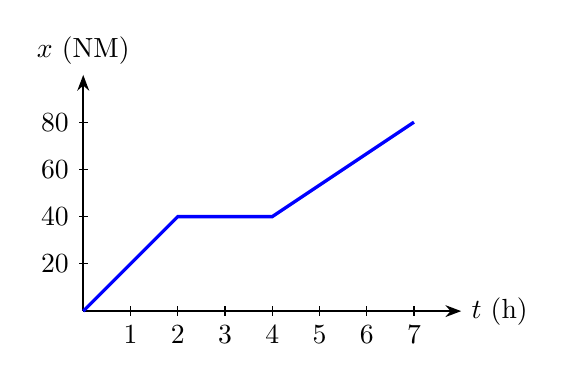
\begin{tikzpicture}[scale=0.6]
\draw[axe, thick] (0,0) -- (8,0) node[right] {$t$ (h)};
\draw[axe, thick] (0,0) -- (0,5) node[above] {$x$ (NM)};
\foreach \x in {1,2,3,4,5,6,7} {\draw (\x,0.1) -- (\x,-0.1) node[below] {\x};}
\foreach \y in {1,2,3,4} {\draw (0.1,\y) -- (-0.1,\y) node[left] {\pgfmathparse{int(\y*20)}\pgfmathresult};}
\draw[very thick, blue] (0,0) -- (2,2) -- (4,2) -- (7,4);
\end{tikzpicture}
\end{center}

\begin{enumerate}[label=\alph*)]
    \item Décrivez qualitativement le mouvement du navire.
    \item Calculez la vitesse entre $t = 0$ et $t = 2$ h.
    \item Le navire est-il à l'arrêt à un certain moment? Si oui, quand?
    \item Quelle est la vitesse moyenne sur l'ensemble du trajet (0 à 7 h)?
\end{enumerate}

\item[$\star\star$] \textbf{15.} Le graphique suivant montre la vitesse d'un cargo en fonction du temps :

\begin{center}
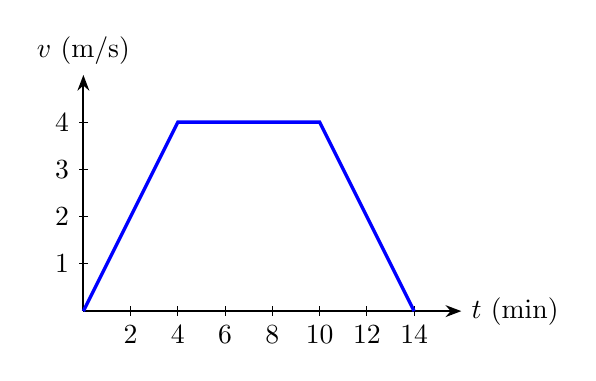
\begin{tikzpicture}[scale=0.6]
\draw[axe, thick] (0,0) -- (8,0) node[right] {$t$ (min)};
\draw[axe, thick] (0,0) -- (0,5) node[above] {$v$ (m/s)};
\foreach \x in {2,4,6,8,10,12,14} {\draw (\x/2,0.1) -- (\x/2,-0.1) node[below] {\x};}
\foreach \y in {1,2,3,4} {\draw (0.1,\y) -- (-0.1,\y) node[left] {\y};}
\draw[very thick, blue] (0,0) -- (2,4) -- (5,4) -- (7,0);
\end{tikzpicture}
\end{center}

\begin{enumerate}[label=\alph*)]
    \item Calculez l'accélération pendant les 4 premières minutes.
    \item Pendant quelle phase le navire est-il en MRU?
    \item Calculez la distance totale parcourue (aire sous la courbe).
\end{enumerate}

\item[$\star\star\star$] \textbf{16.} \textbf{Expliquez} pourquoi, sur un graphique position-temps $x(t)$, une pente négative signifie que l'objet se déplace dans le sens négatif, et non pas qu'il recule nécessairement.

\item[$\star\star$] \textbf{17.} Un navire-citerne effectue une manœuvre d'approche. Le graphique suivant montre sa vitesse en fonction du temps :

\begin{center}
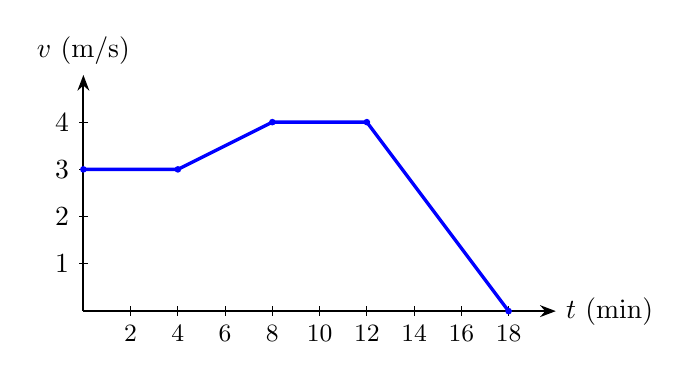
\begin{tikzpicture}[scale=0.6]
\draw[axe, thick] (0,0) -- (10,0) node[right] {$t$ (min)};
\draw[axe, thick] (0,0) -- (0,5) node[above] {$v$ (m/s)};
\foreach \x in {2,4,6,8,10,12,14,16,18} {\draw (\x/2,0.1) -- (\x/2,-0.1) node[below] {\small\x};}
\foreach \y in {1,2,3,4} {\draw (0.1,\y) -- (-0.1,\y) node[left] {\y};}
\draw[very thick, blue] (0,3) -- (2,3) -- (4,4) -- (6,4) -- (9,0);
\fill[blue] (0,3) circle (2pt);
\fill[blue] (2,3) circle (2pt);
\fill[blue] (4,4) circle (2pt);
\fill[blue] (6,4) circle (2pt);
\fill[blue] (9,0) circle (2pt);
\end{tikzpicture}
\end{center}

\begin{enumerate}[label=\alph*)]
    \item Décrivez qualitativement les différentes phases du mouvement.
    \item Calculez l'accélération pendant la phase d'accélération (entre $t = 4$ et $t = 8$ min).
    \item Calculez l'accélération pendant la phase de freinage.
    \item Calculez la distance totale parcourue pendant toute la manœuvre (aire sous la courbe).
    \item \textbf{Tracez} le graphique $a(t)$ correspondant à ce mouvement.
\end{enumerate}

\item[$\star\star\star$] \textbf{18.} Un cargo quitte le port de Montréal. Voici le graphique de son accélération en fonction du temps pendant les 10 premières minutes :

\begin{center}
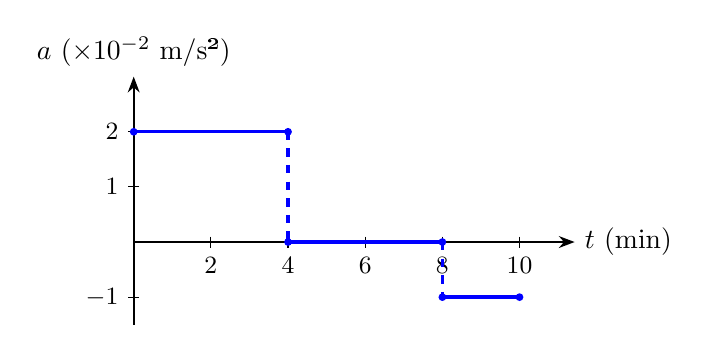
\begin{tikzpicture}[scale=0.7]
\draw[axe, thick] (0,0) -- (8,0) node[right] {$t$ (min)};
\draw[axe, thick] (0,-1.5) -- (0,3) node[above] {$a$ ($\times 10^{-2}$ m/s²)};
% Graduations temps
\foreach \x in {2,4,6,8,10} {\draw (\x*0.7,0.1) -- (\x*0.7,-0.1) node[below] {\small\x};}
% Graduations accélération
\draw (0.1,2) -- (-0.1,2) node[left] {\small 2};
\draw (0.1,1) -- (-0.1,1) node[left] {\small 1};
\draw (0.1,-1) -- (-0.1,-1) node[left] {\small $-1$};
% Courbe: a = 0.02 de 0 à 4 min, puis a = 0 de 4 à 8 min, puis a = -0.01 de 8 à 10 min
\draw[very thick, blue] (0,2) -- (2.8,2);
\draw[very thick, blue, dashed] (2.8,2) -- (2.8,0);
\draw[very thick, blue] (2.8,0) -- (5.6,0);
\draw[very thick, blue, dashed] (5.6,0) -- (5.6,-1);
\draw[very thick, blue] (5.6,-1) -- (7,-1);
\fill[blue] (0,2) circle (2pt);
\fill[blue] (2.8,2) circle (2pt);
\fill[blue] (2.8,0) circle (2pt);
\fill[blue] (5.6,0) circle (2pt);
\fill[blue] (5.6,-1) circle (2pt);
\fill[blue] (7,-1) circle (2pt);
\end{tikzpicture}
\end{center}

Le cargo part du repos ($v_0 = 0$).
\begin{enumerate}[label=\alph*)]
    \item Calculez la vitesse du cargo à $t = 4$ min.
    \item Calculez la vitesse du cargo à $t = 8$ min.
    \item Calculez la vitesse du cargo à $t = 10$ min.
    \item \textbf{Tracez} le graphique $v(t)$ correspondant.
\end{enumerate}

\item[$\star\star\star$] \textbf{19.} Un traversier effectue la traversée entre deux quais. Voici le graphique de sa position en fonction du temps :

\begin{center}
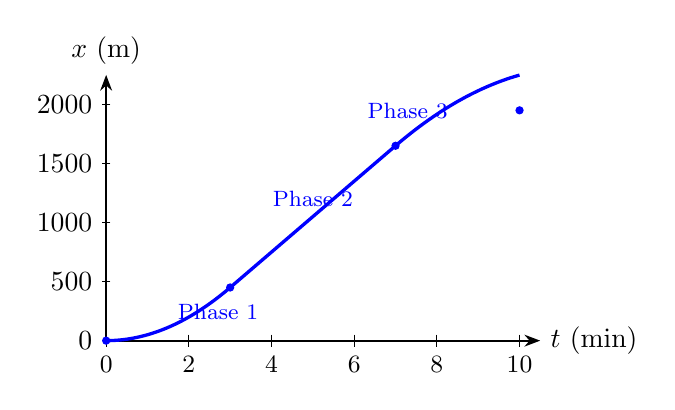
\begin{tikzpicture}[x=0.7cm,y=1cm, scale=0.75]
\draw[axe, thick] (0,0) -- (10.5,0) node[right] {$t$ (min)};
\draw[axe, thick] (0,0) -- (0,4.5) node[above] {$x$ (m)};

% Graduations temps
\foreach \x in {0,2,4,6,8,10} {\draw (\x,0.1) -- (\x,-0.1) node[below] {\small\x};}
% Graduations position (1 unité = 500 m)
\foreach \y in {0,1,2,3,4} {\draw (0.1,\y) -- (-0.1,\y) node[left] {\pgfmathparse{int(\y*500)}\pgfmathresult};}

% Phase 1 : accélération (courbe concave vers le haut) de 0 à 3 min
\draw[very thick, blue, domain=0:3, samples=60] plot (\x, {0.1*\x*\x});

% Phase 2 : vitesse constante (droite) de 3 à 7 min
\draw[very thick, blue] (3,0.9) -- (7,3.3);

% Phase 3 : freinage (courbe concave vers le bas) de 7 à 10 min
\draw[very thick, blue, domain=7:10, samples=80] plot (\x, {3.3 + 0.6*(\x-7) - 0.067*(\x-7)*(\x-7)});

% Points repères
\fill[blue] (0,0) circle (2pt);
\fill[blue] (3,0.9) circle (2pt);
\fill[blue] (7,3.3) circle (2pt);
\fill[blue] (10,3.9) circle (2pt);

% Annotations
\node[above right, blue, font=\footnotesize] at (1.5,0.2) {Phase 1};
\node[above, blue, font=\footnotesize] at (5,2.1) {Phase 2};
\node[above left, blue, font=\footnotesize] at (8.5,3.6) {Phase 3};
\end{tikzpicture}
\end{center}

\begin{enumerate}[label=\alph*)]
    \item Identifiez les trois phases du mouvement (accélération, vitesse constante, freinage).
    \item Estimez graphiquement la vitesse maximale atteinte (pente de la partie linéaire).
    \item Le traversier est-il à l'arrêt au début et à la fin? Justifiez par la forme de la courbe.
    \item \textbf{Tracez} le graphique $v(t)$ correspondant à ce mouvement.
\end{enumerate}

\item[$\star\star\star$] \textbf{19B. Défi -- lecture croisée $x(t)$ et $v(t)$.} On étudie un traversier se déplaçant le long d'un axe $x$ (vers l'est positif). Voici les deux graphiques :

\begin{center}
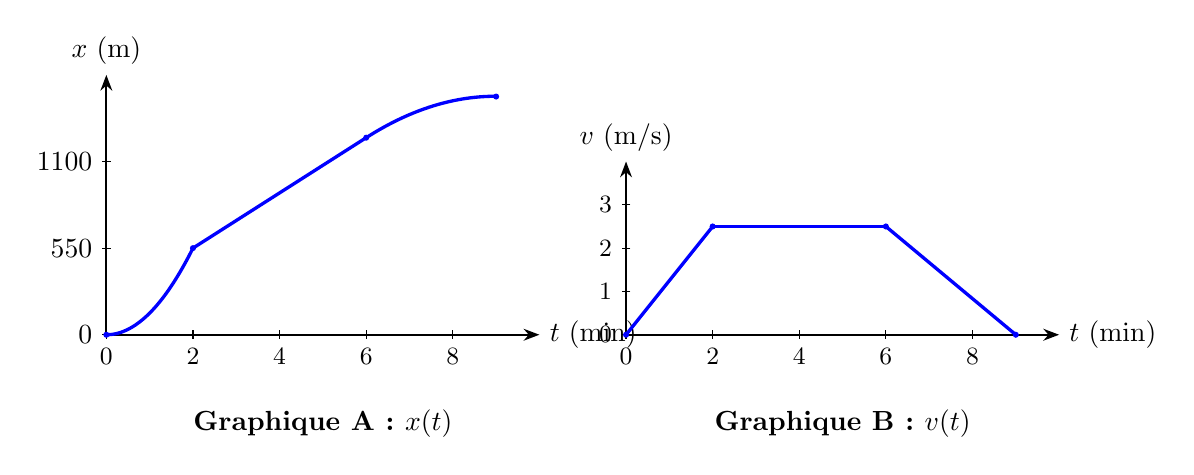
\begin{tikzpicture}[scale=0.55]
% Graphique x(t)
\begin{scope}[xshift=0cm]
\draw[axe, thick] (0,0) -- (10,0) node[right] {$t$ (min)};
\draw[axe, thick] (0,0) -- (0,6) node[above] {$x$ (m)};
\foreach \x in {0,2,4,6,8} {\draw (\x,0.1) -- (\x,-0.1) node[below] {\small\x};}
\foreach \y in {0,2,4} {\draw (0.1,\y) -- (-0.1,\y) node[left] {\pgfmathparse{int(\y*275)}\pgfmathresult};}
% Phase 1 : accélération (0 à 2 min)
\draw[very thick, blue, domain=0:2, samples=40] plot (\x, {0.5*\x*\x});
% Phase 2 : MRU (2 à 6 min)
\draw[very thick, blue] (2,2) -- (6,4.55);
% Phase 3 : freinage (6 à 9 min)
\draw[very thick, blue, domain=6:9, samples=40] plot (\x, {4.55 + 0.64*(\x-6) - 0.107*(\x-6)*(\x-6)});
\fill[blue] (0,0) circle (2pt);
\fill[blue] (2,2) circle (2pt);
\fill[blue] (6,4.55) circle (2pt);
\fill[blue] (9,5.5) circle (2pt);
\node[below] at (5,-1.5) {\textbf{Graphique A : $x(t)$}};
\end{scope}

% Graphique v(t)
\begin{scope}[xshift=12cm]
\draw[axe, thick] (0,0) -- (10,0) node[right] {$t$ (min)};
\draw[axe, thick] (0,0) -- (0,4) node[above] {$v$ (m/s)};
\foreach \x in {0,2,4,6,8} {\draw (\x,0.1) -- (\x,-0.1) node[below] {\small\x};}
\foreach \y in {0,1,2,3} {\draw (0.1,\y) -- (-0.1,\y) node[left] {\small\y};}
% Phase 1 : accélération linéaire
\draw[very thick, blue] (0,0) -- (2,2.5);
% Phase 2 : vitesse constante
\draw[very thick, blue] (2,2.5) -- (6,2.5);
% Phase 3 : décélération linéaire
\draw[very thick, blue] (6,2.5) -- (9,0);
\fill[blue] (0,0) circle (2pt);
\fill[blue] (2,2.5) circle (2pt);
\fill[blue] (6,2.5) circle (2pt);
\fill[blue] (9,0) circle (2pt);
\node[below] at (5,-1.5) {\textbf{Graphique B : $v(t)$}};
\end{scope}
\end{tikzpicture}
\end{center}

\begin{enumerate}[label=\alph*)]
    \item Sur le graphe $x(t)$, à quel(s) instant(s) l'accélération est-elle nulle? Justifiez.
    \item Sur le graphe $v(t)$, indiquez les intervalles où l'accélération est positive, nulle et négative.
    \item Les deux graphes sont-ils compatibles? Donnez deux arguments (pentes et aires).
    \item Sans calculs détaillés, pendant quel intervalle le traversier parcourt-il la plus grande distance : $[0,2]$, $[2,6]$ ou $[6,9]$? Justifiez.
    \item À $t=6$ min, comparez la vitesse instantanée (pente de $x(t)$) et la vitesse moyenne sur $[0,6]$.
\end{enumerate}

\end{enumerate}

% -----------------------------------------------------------------------------
\subsection*{Accélération et MRUA}
% -----------------------------------------------------------------------------

\begin{enumerate}[resume]
\item[$\star$] \textbf{20.} Un porte-conteneurs passe de $\SI{5}{n\oe{}uds}$ à $\SI{18}{n\oe{}uds}$ en $\SI{12}{min}$. Calculez son accélération moyenne en m/s².

\item[$\star$] \textbf{21.} Un TGV roulant à $\SI{320}{km/h}$ freine et s'arrête en $\SI{4}{min}$. Quelle est sa décélération moyenne en m/s²?

\item[$\star\star$] \textbf{22.} Un traversier part du repos et accélère à $\SI{0,08}{m/s^2}$ jusqu'à atteindre $\SI{12}{n\oe{}uds}$.
\begin{enumerate}[label=\alph*)]
    \item Combien de temps dure la phase d'accélération?
    \item Quelle distance parcourt-il pendant cette phase?
\end{enumerate}

\item[$\star\star$] \textbf{23.} Un cargo navigue à $\SI{15}{n\oe{}uds}$. Le capitaine ordonne le freinage avec $a = \SI{-0,006}{m/s^2}$.
\begin{enumerate}[label=\alph*)]
    \item Quelle est la distance de freinage?
    \item Combien de temps faut-il pour s'arrêter?
\end{enumerate}

\item[$\star\star$] \textbf{24.} Une voiture roule à $\SI{90}{km/h}$ et freine avec $a = \SI{-8}{m/s^2}$. Calculez sa distance de freinage. Comparez avec un cargo à la même vitesse qui freine avec $a = \SI{-0,006}{m/s^2}$.

\item[$\star\star\star$] \textbf{25.} Un navire doit s'arrêter exactement à un quai situé à $\SI{800}{m}$. Il arrive à $\SI{8}{n\oe{}uds}$.
\begin{enumerate}[label=\alph*)]
    \item Quelle décélération constante doit-il appliquer?
    \item Combien de temps dure la manœuvre?
    \item Si le capitaine applique plutôt $a = \SI{-0,015}{m/s^2}$, à quelle distance du quai le navire s'arrêtera-t-il?
\end{enumerate}

\item[$\star\star\star$] \textbf{26.} \textbf{Vrai ou faux?} Justifiez.
\begin{enumerate}[label=\alph*)]
    \item Si l'accélération est négative, l'objet ralentit toujours.
    \item Un objet peut avoir une vitesse nulle et une accélération non nulle.
    \item Si la vitesse et l'accélération ont le même signe, l'objet accélère.
\end{enumerate}

\item[$\star\star\star$] \textbf{27.} Deux navires se trouvent à $\SI{3}{km}$ l'un de l'autre et naviguent l'un vers l'autre. Le navire A voyage à vitesse constante de $\SI{8}{n\oe{}uds}$ tandis que le navire B part du repos et accélère à $\SI{0,01}{m/s^2}$.
\begin{enumerate}[label=\alph*)]
    \item Écrivez les équations de position des deux navires (origine au point de départ de A, positif vers B).
    \item Après combien de temps les navires se rencontrent-ils?
    \item À quelle distance du point de départ de A se trouvent-ils?
    \item Quelle est la vitesse de B au moment de la rencontre?
\end{enumerate}

\end{enumerate}

% -----------------------------------------------------------------------------
\subsection*{Chute libre}
% -----------------------------------------------------------------------------

\begin{enumerate}[resume]
\item[$\star$] \textbf{28.} Un matelot échappe un outil du haut d'un mât situé à $\SI{18}{m}$ au-dessus du pont.
\begin{enumerate}[label=\alph*)]
    \item Combien de temps l'outil met-il pour atteindre le pont?
    \item À quelle vitesse frappe-t-il le pont?
\end{enumerate}

\item[$\star$] \textbf{29.} Un ouvrier sur un échafaudage à $\SI{25}{m}$ de hauteur laisse tomber un boulon.
\begin{enumerate}[label=\alph*)]
    \item Combien de temps le boulon met-il pour atteindre le sol?
    \item À quelle vitesse frappe-t-il le sol?
\end{enumerate}

\item[$\star\star$] \textbf{30.} Un marin sur un pont à $\SI{8}{m}$ au-dessus de l'eau lance une bouée de sauvetage verticalement vers le bas avec une vitesse initiale de $\SI{3}{m/s}$.
\begin{enumerate}[label=\alph*)]
    \item Combien de temps la bouée met-elle pour atteindre l'eau?
    \item À quelle vitesse entre-t-elle dans l'eau?
\end{enumerate}

\item[$\star\star$] \textbf{31.} Une fusée éclairante est lancée verticalement vers le haut depuis le pont d'un navire ($y_0 = \SI{5}{m}$) avec une vitesse de $\SI{25}{m/s}$.
\begin{enumerate}[label=\alph*)]
    \item Quelle hauteur maximale atteint-elle au-dessus de l'eau?
    \item Combien de temps reste-t-elle en l'air avant de retomber à l'eau ($y = 0$)?
\end{enumerate}

\item[$\star\star$] \textbf{32.} Un joueur de basketball lance un ballon verticalement vers le haut à $\SI{8}{m/s}$ depuis une hauteur de $\SI{2}{m}$.
\begin{enumerate}[label=\alph*)]
    \item Quelle hauteur maximale le ballon atteint-il?
    \item Combien de temps le ballon reste-t-il en l'air avant de toucher le sol?
\end{enumerate}

\item[$\star\star\star$] \textbf{33.} \textbf{Question contre-intuitive.} Un marin sur un mât laisse tomber une balle A. Au même instant, un autre marin au sol lance une balle B verticalement vers le haut. Les deux balles se croisent à mi-hauteur. 

Laquelle des deux balles a la plus grande vitesse au moment où elles se croisent? \textit{Justifiez sans calcul.}
\end{enumerate}

% -----------------------------------------------------------------------------
\subsection*{Mouvement en 2D et projectile}
% -----------------------------------------------------------------------------

\begin{enumerate}[resume]
\item[$\star$] \textbf{34.} Un navire navigue à $\SI{18}{n\oe{}uds}$ avec un cap de $40°$ nord de l'est.
\begin{enumerate}[label=\alph*)]
    \item Quelle est la composante est-ouest de sa vitesse?
    \item Quelle est la composante nord-sud de sa vitesse?
\end{enumerate}

\item[$\star\star$] \textbf{35.} Un lance-amarre projette une ligne à $\SI{25}{m/s}$ avec un angle de $40°$ depuis une hauteur de $\SI{6}{m}$.
\begin{enumerate}[label=\alph*)]
    \item Calculez les composantes $v_{0x}$ et $v_{0y}$.
    \item Quelle est la portée horizontale?
\end{enumerate}

\item[$\star\star$] \textbf{36.} Un joueur de baseball frappe une balle à $\SI{35}{m/s}$ avec un angle de $30°$ au-dessus de l'horizontale, depuis une hauteur de $\SI{1}{m}$.
\begin{enumerate}[label=\alph*)]
    \item Quelle est la hauteur maximale atteinte par la balle?
    \item Quelle est la portée horizontale?
\end{enumerate}

\item[$\star\star$] \textbf{37.} Un conteneur tombe d'une grue qui se déplace horizontalement à $\SI{2}{m/s}$. Le conteneur est à $\SI{15}{m}$ de hauteur. À quelle distance horizontale (par rapport au point directement sous le largage) le conteneur touche-t-il le sol?

\item[$\star\star\star$] \textbf{38.} Une fusée éclairante est lancée à $\SI{40}{m/s}$ avec un angle de $60°$ depuis le niveau de l'eau.
\begin{enumerate}[label=\alph*)]
    \item Quelle hauteur maximale atteint-elle?
    \item Quelle est sa portée horizontale?
    \item À quel angle faudrait-il la lancer pour maximiser la portée? (Sans calcul)
\end{enumerate}

\item[$\star\star\star$] \textbf{39.} \textbf{Expliquez} pourquoi un objet lancé horizontalement et un objet lâché au même instant depuis la même hauteur touchent le sol en même temps.
\end{enumerate}

% -----------------------------------------------------------------------------
\subsection*{Cinématique de rotation}
% -----------------------------------------------------------------------------

\begin{enumerate}[resume]
\item[$\star$] \textbf{40.} Convertissez : a) $270°$ en radians \quad b) $\frac{3\pi}{4}$~rad en degrés \quad c) $\SI{90}{RPM}$ en rad/s

\item[$\star$] \textbf{41.} Une hélice de navire tourne à $\SI{150}{RPM}$. Si le rayon de l'hélice est de $\SI{2}{m}$, quelle est la vitesse linéaire en bout de pale (en m/s et km/h)?

\item[$\star\star$] \textbf{42.} Un treuil de rayon $\SI{15}{cm}$ doit enrouler $\SI{8}{m}$ de câble.
\begin{enumerate}[label=\alph*)]
    \item Combien de tours doit-il effectuer?
    \item S'il tourne à $\SI{25}{RPM}$, combien de temps faut-il?
\end{enumerate}

\item[$\star\star$] \textbf{43.} L'hélice d'un navire passe de $\SI{0}{RPM}$ à $\SI{120}{RPM}$ en $\SI{20}{s}$ avec une accélération angulaire constante.
\begin{enumerate}[label=\alph*)]
    \item Quelle est l'accélération angulaire en rad/s²?
    \item Combien de tours l'hélice effectue-t-elle pendant cette phase?
\end{enumerate}

\item[$\star\star$] \textbf{44.} Les roues d'une voiture (rayon $\SI{30}{cm}$) tournent à $\SI{800}{RPM}$ lorsque la voiture roule à vitesse constante. Le conducteur freine et la voiture s'arrête après $\SI{50}{m}$.
\begin{enumerate}[label=\alph*)]
    \item Quelle était la vitesse de la voiture?
    \item Quelle est la décélération angulaire des roues?
    \item Combien de tours les roues effectuent-elles pendant le freinage?
\end{enumerate}

\item[$\star\star\star$] \textbf{45.} Un cabestan de rayon $\SI{20}{cm}$ tourne à $\SI{45}{RPM}$. On applique les freins et il s'arrête après 8 tours.
\begin{enumerate}[label=\alph*)]
    \item Quelle est la décélération angulaire?
    \item Quelle longueur de câble a été halée pendant le freinage?
    \item Combien de temps a duré le freinage?
\end{enumerate}
\end{enumerate}

% =============================================================================
\subsection*{Problèmes de synthèse}
% =============================================================================

Ces problèmes intègrent plusieurs concepts du chapitre. Ils sont représentatifs du niveau attendu lors des évaluations.

\begin{enumerate}[resume]
\item[\textbf{S1.}] \textbf{Manœuvre d'accostage}

Un cargo de haute mer arrive au port de Montréal. À $\SI{2}{km}$ du quai, il navigue à $\SI{10}{n\oe{}uds}$. Le pilote du port ordonne une première phase de freinage avec $a_1 = \SI{-0,005}{m/s^2}$ jusqu'à atteindre $\SI{3}{n\oe{}uds}$, puis une seconde phase avec $a_2 = \SI{-0,008}{m/s^2}$ jusqu'à l'arrêt complet.

\begin{enumerate}[label=\alph*)]
    \item Quelle distance parcourt le navire pendant la première phase?
    \item Quelle distance parcourt-il pendant la seconde phase?
    \item Le navire s'arrête-t-il avant le quai? Si non, à quelle distance du quai aurait-il dû commencer à freiner?
\end{enumerate}

\item[\textbf{S2.}] \textbf{Homme à la mer}

Un marin tombe d'un navire qui se déplace à $\SI{14}{n\oe{}uds}$. L'équipage met $\SI{45}{s}$ avant de réagir (temps de réaction), puis le navire freine avec une décélération de $\SI{0,015}{m/s^2}$ jusqu'à l'arrêt.

\begin{enumerate}[label=\alph*)]
    \item Quelle distance le navire parcourt-il pendant le temps de réaction?
    \item Quelle distance parcourt-il pendant le freinage?
    \item À quelle distance totale du point de chute le navire s'arrête-t-il?
    \item Si le marin dérive à $\SI{1}{n\oe{}ud}$ dans le sens opposé au navire, à quelle distance du navire se trouve-t-il quand celui-ci s'arrête?
\end{enumerate}

\item[\textbf{S3.}] \textbf{Sauvetage héliporté}

Un hélicoptère de la Garde côtière vole horizontalement vers l'est à $\SI{90}{km/h}$ à une altitude de $\SI{40}{m}$ au-dessus de l'eau. Il doit larguer une bouée de sauvetage pour qu'elle tombe exactement sur un naufragé.

\begin{enumerate}[label=\alph*)]
    \item À quelle distance horizontale \textbf{avant} le naufragé l'hélicoptère doit-il larguer la bouée?
    \item Avec quelle vitesse (module et direction) la bouée touche-t-elle l'eau?
    \item Si le naufragé dérive vers l'est à $\SI{2}{m/s}$ (même direction que l'hélicoptère), comment cela modifie-t-il la distance de largage?
    \item L'hélicoptère décide plutôt de lancer la bouée vers le bas avec une vitesse initiale de $\SI{5}{m/s}$. Recalculez la distance de largage.
\end{enumerate}

\item[\textbf{S4.}] \textbf{Opération de levage}

Une grue portuaire soulève un conteneur de $\SI{20}{tonnes}$. Le treuil (rayon $\SI{25}{cm}$) accélère de 0 à $\SI{30}{RPM}$ en $\SI{5}{s}$, puis maintient cette vitesse constante.

\begin{enumerate}[label=\alph*)]
    \item Quelle est l'accélération angulaire pendant la phase d'accélération?
    \item À quelle vitesse linéaire le conteneur monte-t-il en régime permanent?
    \item Quelle hauteur le conteneur atteint-il après $\SI{5}{s}$?
    \item Si le câble casse à une hauteur de $\SI{12}{m}$, combien de temps le conteneur met-il pour toucher le sol?
\end{enumerate}

\item[\textbf{S5.}] \textbf{Accident évité de justesse}

Une voiture roule à $\SI{110}{km/h}$ sur l'autoroute. Le conducteur aperçoit un obstacle à $\SI{80}{m}$ devant lui. Son temps de réaction est de $\SI{0,8}{s}$, puis il freine avec une décélération de $\SI{9}{m/s^2}$.

\begin{enumerate}[label=\alph*)]
    \item Quelle distance parcourt la voiture pendant le temps de réaction?
    \item Quelle est la distance de freinage?
    \item La voiture s'arrête-t-elle avant l'obstacle?
\end{enumerate}

\item[\textbf{S6.}] \textbf{Chute d'un grimpeur}

Un grimpeur à $\SI{15}{m}$ au-dessus du sol glisse et tombe en chute libre. Son partenaire d'assurage, au sol, a un temps de réaction de $\SI{0,5}{s}$ avant d'activer le système de freinage qui applique une décélération de $\SI{15}{m/s^2}$ au grimpeur.

\begin{enumerate}[label=\alph*)]
    \item Quelle est la vitesse du grimpeur après $\SI{0,5}{s}$ de chute libre?
    \item Quelle distance a-t-il parcourue pendant ce temps?
    \item Combien de temps supplémentaire faut-il pour l'arrêter complètement?
    \item À quelle hauteur au-dessus du sol le grimpeur s'arrête-t-il?
\end{enumerate}

\item[\textbf{S7.}] \textbf{Course poursuite}

Une voiture de police, initialement à l'arrêt, voit passer un véhicule en infraction à $\SI{120}{km/h}$. Après un temps de réaction de $\SI{2}{s}$, la voiture de police accélère à $\SI{4}{m/s^2}$ jusqu'à atteindre $\SI{160}{km/h}$, vitesse qu'elle maintient ensuite.

\begin{enumerate}[label=\alph*)]
    \item Quelle distance le véhicule en infraction parcourt-il pendant le temps de réaction de la police?
    \item Combien de temps la voiture de police met-elle pour atteindre $\SI{160}{km/h}$?
    \item À quel moment (depuis le passage du véhicule) la police rattrape-t-elle le fuyard?
    \item Quelle distance chaque véhicule a-t-il parcourue?
\end{enumerate}

\item[\textbf{S8.}] \textbf{Évitement de collision}

Deux navires se font face dans un chenal. Le navire A ($\SI{14}{n\oe{}uds}$ vers l'est) et le navire B ($\SI{10}{n\oe{}uds}$ vers l'ouest) sont séparés de $\SI{1500}{m}$. Les deux capitaines freinent simultanément avec des décélérations de $a_A = \SI{-0,008}{m/s^2}$ et $a_B = \SI{-0,005}{m/s^2}$.

\begin{enumerate}[label=\alph*)]
    \item Calculez le temps et la distance de freinage de chaque navire.
    \item Les navires s'arrêtent-ils avant de se percuter?
    \item Si collision il y a, calculez la position de l'impact et les vitesses des navires à ce moment.
    \item Quelle décélération minimale le navire A aurait-il dû appliquer pour éviter la collision (B gardant la même décélération)?
\end{enumerate}

\item[\textbf{S9.}] \textbf{Lancer du poids}

Un athlète lance un poids de $\SI{7,26}{kg}$ avec une vitesse de $\SI{13}{m/s}$ à un angle de $40°$ au-dessus de l'horizontale. Le poids quitte sa main à une hauteur de $\SI{2}{m}$.

\begin{enumerate}[label=\alph*)]
    \item Quelle est la hauteur maximale atteinte par le poids?
    \item Quelle est la portée horizontale (distance officielle du lancer)?
    \item À quel angle le poids devrait-il être lancé pour maximiser la portée?
    \item Si l'athlète pouvait augmenter sa vitesse de lancer de 10\%, de combien la portée augmenterait-elle?
\end{enumerate}

\item[\textbf{S10.}] \textbf{Analyse de navigation}

Un cargo quitte Sept-Îles à 6h00 pour Rimouski ($\SI{180}{NM}$). Il navigue d'abord à $\SI{12}{n\oe{}uds}$ pendant 8 heures, puis accélère à $\SI{0,002}{m/s^2}$ jusqu'à atteindre $\SI{16}{n\oe{}uds}$, vitesse qu'il maintient jusqu'à destination.

\begin{enumerate}[label=\alph*)]
    \item Quelle distance a-t-il parcourue pendant les 8 premières heures?
    \item Combien de temps dure la phase d'accélération?
    \item À quelle heure arrive-t-il à Rimouski?
    \item Tracez le graphique $v(t)$ de ce voyage.
\end{enumerate}

\end{enumerate}

% =============================================================================
\subsection*{Défis intégrateurs}
% =============================================================================

Ces problèmes demandent de combiner plusieurs concepts et de développer une stratégie de résolution. Ils représentent le niveau attendu pour bien maîtriser la cinématique.

\begin{enumerate}
\item[\textbf{D1.}] \textbf{Lance-amarre tactique} $(\star\star\star\star)$

Un officier sur le gaillard d'avant (hauteur $h_1 = \SI{8}{m}$) doit envoyer une amarre sur un quai situé à $\SI{25}{m}$ horizontalement. Le quai est à une hauteur $h_2 = \SI{3}{m}$ au-dessus de l'eau. Le lance-amarre propulse la ligne à $v_0 = \SI{30}{m/s}$.

\begin{enumerate}[label=\alph*)]
    \item Quelle est la différence de hauteur $\Delta y$ entre le point de tir et le point d'arrivée?
    \item Déterminez l'angle minimal $\theta_{min}$ permettant d'atteindre le quai. \textit{(Indice : vous devrez résoudre une équation du second degré en $\tan\theta$)}
    \item Pour cet angle minimal, calculez le temps de vol de l'amarre.
    \item Il existe un deuxième angle $\theta_{max}$ qui permet aussi d'atteindre la cible. Lequel des deux angles est préférable en pratique? Justifiez.
    \item Si le navire s'approche du quai à $\SI{0,5}{m/s}$ pendant le vol de l'amarre, de combien la portée effective est-elle réduite?
\end{enumerate}

\item[\textbf{D2.}] \textbf{Rendez-vous en mer} $(\star\star\star\star)$

Deux navires doivent se rejoindre pour un transfert de personnel. À $t = 0$ :
\begin{itemize}
    \item Le navire A est à l'origine, immobile, et commence à accélérer vers l'est à $\SI{0,02}{m/s^2}$
    \item Le navire B est à $\SI{5}{km}$ à l'est, navigue vers l'ouest à $\SI{8}{n\oe{}uds}$ et maintient cette vitesse
\end{itemize}

\begin{enumerate}[label=\alph*)]
    \item Écrivez les équations de position $x_A(t)$ et $x_B(t)$ pour chaque navire.
    \item À quel instant et à quelle position les navires se rencontrent-ils?
    \item Quelle est la vitesse du navire A au moment du rendez-vous?
    \item Quelle est la vitesse \textbf{relative} du navire A par rapport au navire B à cet instant? Interprétez physiquement.
    \item Si le navire A doit s'arrêter au point de rendez-vous avec une décélération de $\SI{0,015}{m/s^2}$, à quel moment doit-il commencer à freiner?
\end{enumerate}

\item[\textbf{D3.}] \textbf{Analyse complète d'une manœuvre} $(\star\star\star\star)$

Un vraquier de $\SI{200}{m}$ de long effectue la manœuvre suivante dans le chenal :
\begin{itemize}
    \item Phase 1 : Accélération de $\SI{0}{n\oe{}ud}$ à $\SI{6}{n\oe{}uds}$ avec $a_1 = \SI{0,01}{m/s^2}$
    \item Phase 2 : Vitesse constante de $\SI{6}{n\oe{}uds}$ pendant $\SI{15}{min}$
    \item Phase 3 : Accélération de $\SI{6}{n\oe{}uds}$ à $\SI{12}{n\oe{}uds}$ avec $a_3 = \SI{0,008}{m/s^2}$
    \item Phase 4 : Vitesse constante de $\SI{12}{n\oe{}uds}$ jusqu'à destination
\end{itemize}

La destination est à $\SI{10}{km}$ du point de départ.

\begin{enumerate}[label=\alph*)]
    \item Calculez la durée et la distance parcourue pendant chaque phase (1, 2 et 3).
    \item Quelle distance reste-t-il à parcourir en phase 4? Combien de temps dure cette phase?
    \item Calculez le temps total de la manœuvre.
    \item Tracez les graphiques $v(t)$ et $x(t)$ à l'échelle, en identifiant clairement chaque phase.
    \item Calculez la vitesse moyenne sur l'ensemble du trajet. Comparez avec la moyenne arithmétique des vitesses (6 et 12 nœuds).
\end{enumerate}

\item[\textbf{D4.}] \textbf{Système de treuils coordonnés} $(\star\star\star\star)$

Lors d'une opération de chargement, deux treuils travaillent en coordination :
\begin{itemize}
    \item Treuil A (rayon $r_A = \SI{20}{cm}$) : part du repos, accélère à $\alpha_A = \SI{0,5}{rad/s^2}$ pendant $\SI{4}{s}$, puis maintient sa vitesse
    \item Treuil B (rayon $r_B = \SI{30}{cm}$) : tourne à vitesse constante $\omega_B = \SI{2}{rad/s}$ dès $t = 0$
\end{itemize}

Les deux treuils enroulent des câbles reliés au même conteneur par un système de poulies (le conteneur monte à la moyenne des vitesses linéaires des deux câbles).

\begin{enumerate}[label=\alph*)]
    \item Calculez la vitesse angulaire finale du treuil A et sa vitesse linéaire en bout de tambour.
    \item Calculez la vitesse linéaire du câble B.
    \item À $t = \SI{4}{s}$, à quelle vitesse monte le conteneur?
    \item Quelle longueur de câble le treuil A a-t-il enroulée pendant les 4 premières secondes?
    \item Quelle longueur de câble le treuil B a-t-il enroulée pendant le même temps?
    \item De quelle hauteur le conteneur est-il monté pendant ces $\SI{4}{s}$? \textit{(Attention : la vitesse de montée varie!)}
\end{enumerate}

\item[\textbf{D5.}] \textbf{Poursuite et interception} $(\star\star\star\star\star)$

Un navire de patrouille P détecte un navire suspect S à $\SI{8}{km}$ au nord. Au moment de la détection :
\begin{itemize}
    \item Le navire S navigue vers l'est à $\SI{15}{n\oe{}uds}$ (vitesse constante)
    \item Le navire P est immobile mais peut atteindre $\SI{25}{n\oe{}uds}$ avec une accélération de $\SI{0,03}{m/s^2}$
\end{itemize}

Le capitaine de P veut intercepter S en naviguant en ligne droite vers un point d'interception.

\begin{enumerate}[label=\alph*)]
    \item Si P navigue directement vers la position actuelle de S, expliquez pourquoi il ne l'interceptera jamais.
    \item Supposons que P navigue vers un point situé à un angle $\theta$ est du nord. Écrivez les équations de position de P et S en fonction du temps.
    \item Pour une interception, les positions doivent coïncider. Établissez les deux équations (en $x$ et en $y$) qui doivent être satisfaites.
    \item Par essai-erreur ou graphiquement, estimez l'angle $\theta$ optimal et le temps d'interception. \textit{(La solution analytique exacte dépasse le cadre du cours.)}
    \item Quelle distance totale le navire P parcourt-il jusqu'à l'interception?
\end{enumerate}

\item[\textbf{D6.}] \textbf{Chute d'un conteneur en mouvement} $(\star\star\star\star)$

Une grue portuaire déplace un conteneur horizontalement à $\SI{3}{m/s}$ à une hauteur de $\SI{20}{m}$. Le câble casse et le conteneur tombe.

\begin{enumerate}[label=\alph*)]
    \item Combien de temps le conteneur met-il pour toucher le sol?
    \item À quelle distance horizontale du point de rupture le conteneur atterrit-il?
    \item Avec quelle vitesse (module) le conteneur frappe-t-il le sol?
    \item Un travailleur se trouve à $\SI{8}{m}$ horizontalement du point de rupture (dans la direction du mouvement). A-t-il le temps de s'écarter s'il lui faut $\SI{1,5}{s}$ pour réagir et courir $\SI{3}{m}$?
    \item Le conteneur a des dimensions $\SI{6}{m} \times \SI{2,4}{m}$ (longueur $\times$ largeur). En supposant qu'il ne tourne pas pendant la chute, quelle est la \og zone de danger \fg{} au sol (rectangle où le conteneur pourrait tomber)?
\end{enumerate}

\item[\textbf{D7.}] \textbf{Navigation avec courant variable} $(\star\star\star\star\star)$

Un navire doit traverser un détroit de $\SI{4}{km}$ de large (direction nord-sud). Le courant dans le détroit varie linéairement :
\begin{itemize}
    \item Au bord sud : courant nul
    \item Au centre : courant maximal de $\SI{3}{n\oe{}uds}$ vers l'est
    \item Au bord nord : courant nul
\end{itemize}

Le navire part du bord sud et navigue à $\SI{10}{n\oe{}uds}$ (vitesse surface) cap au nord.

\begin{enumerate}[label=\alph*)]
    \item Exprimez le courant $v_c(y)$ en fonction de la position $y$ (où $y = 0$ au sud et $y = \SI{4}{km}$ au nord).
    \item Expliquez qualitativement pourquoi le navire dérivera vers l'est, puis reviendra partiellement.
    \item À quelle distance à l'est de sa ligne de départ le navire se trouvera-t-il quand il atteindra le bord nord? \textit{(Indice : divisez la traversée en petits segments et sommez les dérives, ou utilisez l'intégration si vous la connaissez.)}
    \item Combien de temps dure la traversée?
    \item Quel cap initial (ouest du nord) le capitaine devrait-il prendre pour arriver exactement au point visé? \textit{(Question ouverte -- une réponse approximative est acceptable.)}
\end{enumerate}

\item[\textbf{D8.}] \textbf{Interception 2D avec accélération} $(\star\star\star\star\star)$

Un cargo navigue vers l'est à vitesse constante de $\SI{12}{n\oe{}uds}$. Un garde-côte, situé $\SI{800}{m}$ au sud de la trajectoire du cargo et exactement à la même longitude (vis-à-vis de sa position actuelle), doit l'intercepter. Le garde-côte peut accélérer à $\SI{0,03}{m/s^2}$ jusqu'à une vitesse maximale de $\SI{25}{n\oe{}uds}$.

\begin{enumerate}[label=\alph*)]
    \item Si le garde-côte navigue directement vers le nord (perpendiculairement), interceptera-t-il le cargo? Justifiez.
    \item Le garde-côte décide de naviguer avec un angle $\theta$ est du nord. Écrivez les équations de position des deux navires (origine à la position initiale du garde-côte).
    \item Pour un angle de $30°$ est du nord, calculez le temps nécessaire au garde-côte pour atteindre la trajectoire du cargo (la ligne est-ouest à $y = \SI{800}{m}$).
    \item Pour ce même angle, le cargo sera-t-il encore là? Comparez les positions horizontales des deux navires à cet instant.
    \item \textit{(Question ouverte)} Estimez graphiquement ou par essai-erreur l'angle optimal pour minimiser le temps d'interception.
\end{enumerate}

\item[\textbf{D9.}] \textbf{Manœuvre d'accostage optimale} $(\star\star\star\star)$

Un traversier doit rejoindre un quai situé à exactement $\SI{2}{km}$. Pour le confort des passagers, le capitaine souhaite une manœuvre symétrique : accélérer uniformément pendant la première moitié de la distance, puis freiner uniformément (avec la même magnitude d'accélération) pour s'arrêter exactement au quai.

\begin{enumerate}[label=\alph*)]
    \item Si l'accélération est de $\SI{0,04}{m/s^2}$, quelle est la vitesse maximale atteinte (à mi-parcours)?
    \item Quel est le temps total de la manœuvre?
    \item Comparez ce temps avec celui d'un trajet à vitesse constante égale à la vitesse moyenne de cette manœuvre.
    \item Le capitaine réalise qu'il peut accélérer à $\SI{0,06}{m/s^2}$ mais ne peut freiner qu'à $\SI{0,04}{m/s^2}$. À quelle distance du quai doit-il commencer à freiner? Quelle est la nouvelle vitesse maximale?
    \item Pour cette manœuvre asymétrique, calculez le nouveau temps total et comparez avec la manœuvre symétrique.
\end{enumerate}

\end{enumerate}

\bigskip
\begin{remarque}[title=Conseils pour les défis]
\begin{itemize}
    \item \textbf{Dessinez toujours} un schéma avec les axes, les positions initiales et les directions.
    \item \textbf{Identifiez les phases} du mouvement (MRU, MRUA, chute libre...) pour chaque objet.
    \item \textbf{Listez les inconnues} et comptez vos équations -- vous devez avoir autant d'équations que d'inconnues.
    \item \textbf{Le temps est souvent le lien} entre les composantes $x$ et $y$, ou entre deux objets.
    \item \textbf{Vérifiez vos unités} à chaque étape et la cohérence de vos réponses (ordres de grandeur).
\end{itemize}
\end{remarque}

% =============================================================================
\subsection*{Réponses}
% =============================================================================

\textbf{Position et déplacement}

\textbf{1.} a) $\SI{22}{km}$ \quad b) $\SI{+8}{km}$ vers l'est

\textbf{2.} $d = \SI{650}{m}$, $\Delta x = \SI{+350}{m}$ vers l'est

\textbf{3.} a) $\SI{17}{km}$ \quad b) $|\Delta\vec{r}| = \SI{13}{km}$

\textbf{4.} a) Faux (égalité si ligne droite sans demi-tour) \quad b) Vrai \quad c) Faux (ne dépend que des positions initiale et finale)

\medskip
\textbf{Vitesse moyenne et scalaire}

\textbf{5.} $\SI{27,3}{km/h}$ ; $\SI{7,58}{m/s}$ ; $\SI{14,7}{n\oe{}uds}$

\textbf{6.} $\SI{15}{n\oe{}uds}$ ; $\SI{7,72}{m/s}$

\textbf{7.} a) $\SI{4,67}{h}$ \quad b) $\SI{0}{n\oe{}ud}$ \quad c) $\SI{17,1}{n\oe{}uds}$

\textbf{8.} $\SI{13,3}{n\oe{}uds}$

\textbf{9.} a) $\SI{13,3}{n\oe{}uds}$ \quad b) Le temps passé à chaque vitesse n'est pas égal

\textbf{10.} $\SI{15}{n\oe{}uds}$ (moyenne arithmétique car temps égaux)

\textbf{11.} a) $\SI{1,0}{h} = \SI{60}{min}$ \quad b) $\SI{90}{km}$ de la gare A

\textbf{12.} a) $\approx$ 10h43 \quad b) $\SI{171}{km}$ de Montréal

\textbf{13.} a) $\SI{2,3}{min} \approx \SI{138}{s}$ \quad b) Cycliste : $\SI{962}{m}$ ; Coureur : $\SI{462}{m}$

\medskip
\textbf{Graphiques}

\textbf{14.} a) MRU, repos, MRU \quad b) $\SI{20}{NM/h}$ \quad c) Oui, entre 2h et 4h \quad d) $\SI{11,4}{NM/h}$

\textbf{15.} a) $\SI{1}{m/s/min} = \SI{0,017}{m/s^2}$ \quad b) Entre 4 et 10 min \quad c) $\SI{1680}{m}$

\textbf{16.} Le signe dépend du choix de l'axe; une pente négative indique un mouvement vers les $x$ décroissants

\medskip
\textbf{Accélération et MRUA}

\textbf{20.} $\SI{0,0093}{m/s^2}$

\textbf{21.} $\SI{-0,37}{m/s^2}$

\textbf{22.} a) $\SI{77}{s}$ \quad b) $\SI{238}{m}$

\textbf{23.} a) $\SI{4940}{m} \approx \SI{2,7}{NM}$ \quad b) $\SI{1286}{s} \approx \SI{21}{min}$

\textbf{24.} Voiture : $\SI{39}{m}$ ; Cargo : $\SI{52\,000}{m}$ (1300 fois plus!)

\textbf{25.} a) $\SI{-0,0106}{m/s^2}$ \quad b) $\SI{389}{s}$ \quad c) $\SI{234}{m}$ avant le quai

\textbf{26.} a) Faux (dépend du signe de $v$) \quad b) Vrai (ex: balle au sommet) \quad c) Vrai

\textbf{27.} a) $x_A = 4{,}12t$ ; $x_B = 3000 - 0{,}005t^2$ \quad b) $\SI{403}{s} \approx \SI{6,7}{min}$ \quad c) $\SI{1660}{m}$ de A \quad d) $\SI{4,0}{m/s} \approx \SI{7,8}{n\oe{}uds}$

\medskip
\textbf{Chute libre}

\textbf{28.} a) $\SI{1,92}{s}$ \quad b) $\SI{18,8}{m/s}$

\textbf{29.} a) $\SI{2,26}{s}$ \quad b) $\SI{22,1}{m/s}$

\textbf{30.} a) $\SI{1,05}{s}$ \quad b) $\SI{13,3}{m/s}$

\textbf{31.} a) $\SI{36,9}{m}$ \quad b) $\SI{5,3}{s}$

\textbf{32.} a) $\SI{5,27}{m}$ \quad b) $\SI{1,85}{s}$

\textbf{33.} La balle B (lancée) a une plus grande vitesse car elle a eu le temps d'accélérer depuis le sol

\medskip
\textbf{Mouvement en 2D et projectile}

\textbf{34.} a) $\SI{13,8}{n\oe{}uds}$ \quad b) $\SI{11,6}{n\oe{}uds}$

\textbf{35.} a) $v_{0x} = \SI{19,2}{m/s}$, $v_{0y} = \SI{16,1}{m/s}$ \quad b) $\SI{69}{m}$

\textbf{36.} a) $\SI{16,6}{m}$ \quad b) $\SI{109}{m}$

\textbf{37.} $\SI{3,5}{m}$

\textbf{38.} a) $\SI{61,2}{m}$ \quad b) $\SI{141}{m}$ \quad c) $45°$

\textbf{39.} Le mouvement vertical est indépendant du mouvement horizontal; les deux subissent la même accélération $g$

\medskip
\textbf{Cinématique de rotation}

\textbf{40.} a) $\frac{3\pi}{2} \approx \SI{4,71}{rad}$ \quad b) $135°$ \quad c) $\SI{9,42}{rad/s}$

\textbf{41.} $\SI{31,4}{m/s} \approx \SI{113}{km/h}$

\textbf{42.} a) $8,5$ tours \quad b) $\SI{20,4}{s}$

\textbf{43.} a) $\SI{0,628}{rad/s^2}$ \quad b) $20$ tours

\textbf{44.} a) $\SI{25,1}{m/s} \approx \SI{90}{km/h}$ \quad b) $\SI{-6,3}{rad/s^2}$ \quad c) $26,5$ tours

\textbf{45.} a) $\SI{-0,221}{rad/s^2}$ \quad b) $\SI{10,1}{m}$ \quad c) $\SI{21,3}{s}$

\medskip
\textbf{Problèmes de synthèse}

\textbf{S1.} a) $\SI{1890}{m}$ \quad b) $\SI{118}{m}$ \quad c) Non, s'arrête à $\SI{8}{m}$ avant; aurait dû commencer à $\SI{2008}{m}$

\textbf{S2.} a) $\SI{324}{m}$ \quad b) $\SI{173}{m}$ \quad c) $\SI{497}{m}$ \quad d) $\SI{521}{m}$

\textbf{S3.} a) $\SI{71,4}{m}$ \quad b) $v = \SI{37,5}{m/s}$ à $41,8°$ sous l'horizontale \quad c) Réduit de $\SI{5,7}{m}$ (larguer à $\SI{65,7}{m}$) \quad d) $\SI{63,9}{m}$

\textbf{S4.} a) $\SI{0,628}{rad/s^2}$ \quad b) $\SI{0,785}{m/s}$ \quad c) $\SI{0,98}{m}$ \quad d) $\SI{1,56}{s}$

\textbf{S5.} a) $\SI{24,4}{m}$ \quad b) $\SI{52}{m}$ \quad c) Oui, s'arrête à $\SI{3,6}{m}$ de l'obstacle \quad d) $\SI{19,4}{m/s} \approx \SI{70}{km/h}$

\textbf{S6.} a) $\SI{4,9}{m/s}$ \quad b) $\SI{1,23}{m}$ \quad c) $\SI{0,33}{s}$ \quad d) $\SI{12,97}{m}$ (s'arrête à environ $\SI{13}{m}$)

\textbf{S7.} a) $\SI{66,7}{m}$ \quad b) $\SI{11,1}{s}$ \quad c) $t \approx \SI{38}{s}$ \quad d) Police : $\SI{1270}{m}$ ; Fuyard : $\SI{1270}{m}$

\textbf{S8.} a) $A$: $t = \SI{901}{s}$, $d = \SI{3246}{m}$ ; $B$: $t = \SI{1029}{s}$, $d = \SI{2646}{m}$ \quad b) Non, collision \quad c) Position $\approx \SI{940}{m}$ de A; $v_A \approx \SI{4,6}{m/s}$, $v_B \approx \SI{3,2}{m/s}$ \quad d) $a_A \geq \SI{-0,035}{m/s^2}$

\textbf{S9.} a) $\SI{5,55}{m}$ \quad b) $\SI{17,8}{m}$ \quad c) $\approx 42°$ (légèrement moins que 45° car lancé en hauteur) \quad d) Portée augmente de $\approx 21\%$ (proportionnel à $v^2$)

\textbf{S10.} a) $\SI{96}{NM}$ \quad b) $\SI{1029}{s} \approx \SI{17}{min}$ \quad c) $\approx$ 17h30 \quad d) Graphique trapézoïdal

\medskip
\textbf{Défis intégrateurs}

\textbf{D1.} a) $\Delta y = \SI{+5}{m}$ (tire vers le bas) \quad b) $\theta_{min} \approx 28°$ \quad c) $t \approx \SI{1,4}{s}$ \quad d) $\theta_{min}$ préférable (trajectoire plus tendue, moins affectée par le vent) \quad e) Portée réduite de $\SI{0,7}{m}$

\textbf{D2.} a) $x_A = \frac{1}{2}(0,02)t^2$; $x_B = 5000 - 4,12t$ \quad b) $t = \SI{650}{s}$, $x = \SI{4220}{m}$ \quad c) $\SI{13}{m/s} = \SI{25,3}{n\oe{}uds}$ \quad d) $v_{A/B} = \SI{17,1}{m/s}$ vers l'est (A s'approche rapidement de B) \quad e) Commencer à freiner à $t = \SI{217}{s}$

\textbf{D3.} a) Phase 1: $\SI{309}{s}$, $\SI{476}{m}$; Phase 2: $\SI{900}{s}$, $\SI{2778}{m}$; Phase 3: $\SI{386}{s}$, $\SI{1736}{m}$ \quad b) $\SI{5010}{m}$ restants, $\SI{811}{s}$ \quad c) $\SI{2406}{s} \approx \SI{40}{min}$ \quad d) Voir graphique \quad e) $v_{moy} = \SI{15,0}{km/h} = \SI{8,1}{n\oe{}uds}$ (inférieure à $\SI{9}{n\oe{}uds}$, moyenne arithmétique)

\textbf{D4.} a) $\omega_A = \SI{2}{rad/s}$, $v_A = \SI{0,4}{m/s}$ \quad b) $v_B = \SI{0,6}{m/s}$ \quad c) $v_{cont} = \SI{0,5}{m/s}$ \quad d) $L_A = \SI{0,8}{m}$ \quad e) $L_B = \SI{2,4}{m}$ \quad f) $h = \SI{1,33}{m}$ (intégration de la vitesse moyenne)

\textbf{D5.} a) S se déplace; quand P atteint la position initiale de S, celui-ci est déjà ailleurs \quad b) $x_P = v_P(t)\sin\theta \cdot t$; $y_P = v_P(t)\cos\theta \cdot t$; $x_S = 7,72t$; $y_S = 8000$ \quad c) $x_P = x_S$ et $y_P = y_S$ \quad d) $\theta \approx 50°$ est du nord, $t \approx \SI{620}{s}$ \quad e) $\approx \SI{6,2}{km}$

\textbf{D6.} a) $\SI{2,02}{s}$ \quad b) $\SI{6,06}{m}$ \quad c) $\SI{20,0}{m/s}$ \quad d) Non! Le conteneur atterrit à $\SI{6,06}{m}$, le travailleur à $\SI{8}{m}$ est en sécurité même sans bouger \quad e) Zone de $\SI{6}{m} \times \SI{2,4}{m}$ centrée à $\SI{6,06}{m}$ du point de rupture (de $\SI{3,06}{m}$ à $\SI{9,06}{m}$)

\textbf{D7.} a) $v_c(y) = \SI{3}{nd} \times \sin\left(\frac{\pi y}{\SI{4}{km}}\right)$ ou approximation triangulaire \quad b) Dérive maximale au centre où le courant est maximal, puis le courant diminue mais ne ramène pas le navire \quad c) $\approx \SI{780}{m}$ vers l'est \quad d) $\SI{24}{min}$ \quad e) $\approx 5°$ à $7°$ ouest du nord (solution itérative)

\textbf{D8.} a) Non, le cargo se sera déplacé vers l'est pendant que le garde-côte monte vers le nord \quad b) $x_{GC} = \frac{1}{2}(0,03)t^2 \sin\theta$, $y_{GC} = \frac{1}{2}(0,03)t^2 \cos\theta$; $x_C = 6,17t$, $y_C = 800$ \quad c) $t \approx \SI{264}{s}$ pour atteindre $y = 800$ m \quad d) $x_{GC} \approx \SI{523}{m}$, $x_C \approx \SI{1629}{m}$ -- le cargo est loin devant \quad e) $\theta \approx 55°$ à $60°$ est du nord

\textbf{D9.} a) $v_{max} = \SI{8,94}{m/s} \approx \SI{17,4}{n\oe{}uds}$ \quad b) $t_{total} = \SI{447}{s} \approx \SI{7,5}{min}$ \quad c) Vitesse moyenne = $\SI{4,47}{m/s}$; à vitesse constante : $t = \SI{447}{s}$ (identique!) \quad d) Freiner à $\SI{800}{m}$ du quai; $v_{max} = \SI{9,80}{m/s}$ \quad e) $t_{total} = \SI{408}{s} \approx \SI{6,8}{min}$ (plus rapide de 9\%)
\end{frame}

\section{Chapitre 2 -- Dynamique et statique}
\begin{frame}[allowframebreaks]{Exercices (chapitre 2)}
  % =============================================================================
% EXERCICES — CHAPITRE 2 : DYNAMIQUE ET STATIQUE
% =============================================================================

\section*{Exercices}
\addcontentsline{toc}{section}{Exercices}
\begin{remarque}[title=Niveaux de difficulté]
\begin{itemize}
    \item[$\star$] Application directe d'une formule
    \item[$\star\star$] Problème à plusieurs étapes ou avec conversion
    \item[$\star\star\star$] Problème complexe ou piège conceptuel
\end{itemize}
\end{remarque}

\textbf{Données utiles :}
\begin{itemize}
    \item Accélération gravitationnelle : $g = \SI{9,81}{m/s^2}$
    \item Constante de gravitation : $G = \SI{6,674e-11}{N \cdot m^2/kg^2}$
    \item Masse de la Terre : $M_T = \SI{5,972e24}{kg}$
    \item Rayon de la Terre : $R_T = \SI{6,378e6}{m}$
    \item 1 nœud $= \SI{0,514}{m/s}$
\end{itemize}

% =============================================================================
\subsection*{A — Concepts fondamentaux et lois de Newton}
% =============================================================================

\begin{enumerate}

% ---- EXERCICE 1 — Vrai ou faux conceptuel ★ --------------------------------
\item[$\star$] \textbf{1. Vrai ou faux.} Pour chaque affirmation, indiquez si elle est vraie ou fausse et \textbf{justifiez} votre réponse en une ou deux phrases.

\begin{enumerate}[label=\alph*)]
    \item Si aucune force nette n'agit sur un objet, celui-ci est nécessairement immobile.
    \item Un navire qui se déplace à vitesse constante en eau calme n'a aucune force qui agit sur lui.
    \item Un objet plus lourd tombe plus vite qu'un objet plus léger (en négligeant la résistance de l'air).
    \item Lorsqu'un remorqueur pousse un navire, le navire exerce sur le remorqueur une force de réaction plus petite, car le navire est plus massif.
    \item La force normale exercée par une surface sur un objet est toujours égale au poids de cet objet.
    \item Si la force résultante sur un objet est nulle, la vitesse de cet objet est nécessairement nulle.
\end{enumerate}

\textit{Réponses :}
\begin{enumerate}[label=\alph*)]
    \item \textbf{Faux.} Selon la première loi de Newton, si la force nette est nulle, l'objet conserve son état de mouvement : il peut être immobile \textit{ou} se déplacer à vitesse constante (MRU).
    \item \textbf{Faux.} Les forces sont présentes (poids, poussée d'Archimède, poussée des moteurs, résistance de l'eau), mais leur somme vectorielle est nulle. C'est un état d'équilibre dynamique.
    \item \textbf{Faux.} La deuxième loi donne $a = F_g/m = mg/m = g$. L'accélération gravitationnelle est la même pour tous les objets, indépendamment de leur masse.
    \item \textbf{Faux.} Selon la troisième loi de Newton, les forces d'action et de réaction sont \textit{toujours} égales en grandeur et opposées en direction, peu importe les masses des objets.
    \item \textbf{Faux.} La normale est égale au poids uniquement sur une surface horizontale sans autres forces verticales. Sur un plan incliné ou si une force a une composante verticale, $N \neq mg$.
    \item \textbf{Faux.} C'est une reformulation du (a). Force résultante nulle signifie accélération nulle, pas vitesse nulle.
\end{enumerate}

% ---- EXERCICE 2 — Identification des forces ★ ------------------------------
\item[$\star$] \textbf{2. Identification des forces.} Pour chacune des situations suivantes, identifiez \textbf{toutes} les forces qui agissent sur l'objet souligné et indiquez leur direction. Ne faites aucun calcul.

\begin{enumerate}[label=\alph*)]
    \item Un \underline{conteneur} est posé sur le pont d'un navire en mer calme. Le navire se déplace à vitesse constante.
    \item Un \underline{navire} est tiré par un remorqueur à vitesse constante dans un port.
    \item Une \underline{caisse} est tirée sur un quai par un câble formant un angle au-dessus de l'horizontale. La caisse accélère et il y a du frottement cinétique.
    \item Un \underline{conteneur} est suspendu, immobile, au câble d'une grue au-dessus du quai.
\end{enumerate}

\textit{Réponses :}
\begin{enumerate}[label=\alph*)]
    \item \textbf{Conteneur sur le pont :} poids $\vect{F}_g$ (vers le bas) et force normale $\vect{N}$ du pont (vers le haut). Deux forces.
    \item \textbf{Navire remorqué :} poids $\vect{F}_g$ (vers le bas), poussée d'Archimède $\vect{F}_A$ (vers le haut), tension du câble de remorquage $\vect{T}$ (vers l'avant), résistance de l'eau $\vect{f}$ (vers l'arrière). Quatre forces. (La somme est nulle puisque $v$ = constante.)
    \item \textbf{Caisse tirée :} poids $\vect{F}_g$ (vers le bas), force normale $\vect{N}$ (vers le haut), tension $\vect{T}$ (à angle vers le haut et l'avant), frottement cinétique $\vect{f}_c$ (vers l'arrière, parallèle à la surface). Quatre forces. (La somme n'est pas nulle : la caisse accélère.)
    \item \textbf{Conteneur suspendu :} poids $\vect{F}_g$ (vers le bas) et tension du câble $\vect{T}$ (vers le haut). Deux forces. ($T = F_g$ en équilibre.)
\end{enumerate}

% ---- EXERCICE 3 — Paires action-réaction ★ ---------------------------------
\item[$\star$] \textbf{3. Paires action-réaction (3\textsuperscript{e} loi de Newton).} Pour chaque force ci-dessous, identifiez la force de réaction : sur quel objet s'exerce-t-elle, par quel objet est-elle exercée, et dans quelle direction agit-elle?

\begin{enumerate}[label=\alph*)]
    \item La Terre exerce une force gravitationnelle vers le \textit{bas} sur un navire.
    \item L'hélice d'un navire pousse l'eau vers l'\textit{arrière}.
    \item Une amarre exerce une tension sur le navire, dirigée vers le quai.
    \item Le pont du navire exerce une force normale vers le \textit{haut} sur un conteneur.
\end{enumerate}

\textit{Réponses :}
\begin{enumerate}[label=\alph*)]
    \item \textbf{Réaction :} Le navire exerce une force gravitationnelle vers le \textit{haut} sur la Terre. (Même grandeur, mais totalement négligeable pour la Terre vu sa masse énorme.)
    \item \textbf{Réaction :} L'eau pousse l'hélice (et donc le navire) vers l'\textit{avant}. C'est cette réaction qui propulse le navire!
    \item \textbf{Réaction :} Le navire exerce une tension sur l'amarre, dirigée \textit{vers le large} (opposée à la direction du quai).
    \item \textbf{Réaction :} Le conteneur exerce une force vers le \textit{bas} sur le pont du navire. (C'est le « poids apparent » du conteneur sur le pont.)
\end{enumerate}

\end{enumerate}

% =============================================================================
\subsection*{B — Diagramme de corps libre et équilibre (statique)}
% =============================================================================

\begin{enumerate}[resume]

% ---- EXERCICE 4 — Tracé de DCL (sans calcul) ★ -----------------------------
\item[$\star$] \textbf{4. Tracé de DCL (sans calcul).} Pour chacune des situations suivantes, tracez le diagramme de corps libre (DCL) de l'objet indiqué. Identifiez chaque force par son symbole, indiquez sa direction et précisez l'objet qui l'exerce.

\begin{enumerate}[label=\alph*)]
    \item Un moteur de \SI{250}{kg} est suspendu au plafond de la salle des machines par un câble vertical unique.
    \item Une caisse de \SI{100}{kg} est immobile sur une rampe de chargement inclinée à $30°$, retenue par le frottement statique.
    \item Un conteneur est retenu en l'air par deux câbles : le premier fait un angle de $20°$ avec la verticale et le second fait un angle de $45°$ avec la verticale.
\end{enumerate}

\textit{Réponses :}
\begin{enumerate}[label=\alph*)]
    \item Deux forces : poids $\vect{F}_g$ (vers le bas) et tension $\vect{T}$ (vers le haut). Le point d'application est le centre de masse du moteur.
    \item Trois forces : poids $\vect{F}_g$ (verticalement vers le bas, au centre de masse), force normale $\vect{N}$ (perpendiculaire à la rampe, vers l'extérieur de la surface) et frottement statique $\vect{f}_s$ (parallèle à la rampe, vers le haut de la pente).
    \item Trois forces : poids $\vect{F}_g$ (vers le bas) et deux tensions $\vect{T}_1$ (le long du premier câble, à $20°$ de la verticale) et $\vect{T}_2$ (le long du second câble, à $45°$ de la verticale).
\end{enumerate}

% ---- EXERCICE 5 — Câbles dans la salle des machines ★★ ---------------------
\item[$\star\star$] \textbf{5. (Maritime)} Un moteur diesel de \SI{300}{kg} est suspendu au point de jonction A par un câble vertical dans la salle des machines d'un navire. Au point A, deux câbles maintiennent le système en équilibre :
\begin{itemize}
    \item le câble AB est fixé au plafond et fait un angle de $40°$ avec l'horizontale;
    \item le câble AD est horizontal et fixé à une cloison.
\end{itemize}

\begin{center}
\begin{tikzpicture}[scale=1.0, >=Stealth]
    % --- Coordonnées ---
    \coordinate (A) at (0, 0);
    \coordinate (B) at ({-3.5*cos(40)}, {3.5*sin(40)});
    \coordinate (D) at (3.2, 0);
    % --- Plafond ---
    \pgfmathsetmacro{\yPlaf}{3.5*sin(40)}
    \fill[pattern=north east lines, pattern color=gray!60] 
        ({-3.5*cos(40) - 0.5}, \yPlaf) rectangle (3.5, {\yPlaf + 0.3});
    \draw[thick] ({-3.5*cos(40) - 0.5}, \yPlaf) -- (3.5, \yPlaf);
    % --- Cloison droite ---
    \fill[pattern=north east lines, pattern color=gray!60] 
        (3.2, -2.6) rectangle (3.5, \yPlaf);
    \draw[thick] (3.2, -2.6) -- (3.2, \yPlaf);
    % --- Câble AB ---
    \draw[thick] (A) -- (B);
    \node[above left=2pt] at ($(A)!0.55!(B)$) {$T_{AB}$};
    % --- Câble AD ---
    \draw[thick] (A) -- (D);
    \node[above=3pt] at ($(A)!0.5!(D)$) {$T_{AD}$};
    % --- Câble vertical ---
    \draw[thick] (A) -- (0, -1.5);
    % --- Point A ---
    \filldraw[black] (A) circle (2.5pt);
    \node[below left=4pt] at (A) {A};
    % --- Points B et D ---
    \filldraw[black] (B) circle (2pt);
    \node[below left=2pt, font=\small] at (B) {B};
    \filldraw[black] (D) circle (2pt);
    \node[above left=2pt, font=\small] at (D) {D};
    % --- Angle 40° ---
    \draw[dashed, gray] (A) -- +(-2.8, 0);
    \draw[thick, blue!70] ($(A) + (180:0.9)$) arc (180:140:0.9);
    \node[blue!70, font=\small] at ($(A) + (160:1.25)$) {$40^\circ$};
    % --- Moteur ---
    \draw[thick, fill=gray!25] (-0.7, -2.3) rectangle (0.7, -1.5);
    \node at (0, -1.9) {M};
    \node[below, font=\small] at (0, -2.4) {\SI{300}{kg}};
\end{tikzpicture}
\end{center}

\begin{enumerate}[label=\alph*)]
    \item Tracez le DCL du point A.
    \item Déterminez la tension dans le câble AB.
    \item Déterminez la tension dans le câble AD.
\end{enumerate}

\textit{Réponses : b) $T_{AB} = \SI{4,58}{kN}$ \quad c) $T_{AD} = \SI{3,51}{kN}$}

% ---- EXERCICE 6 — Grue de chargement ★★ ------------------------------------
\item[$\star\star$] \textbf{6. (Maritime)} Un conteneur de \SI{2500}{kg} est soulevé par la grue d'un navire. Le câble de la grue fait un angle de $20°$ avec la verticale. Une amarre horizontale est attachée au conteneur pour l'empêcher de balancer.

\begin{center}
\begin{tikzpicture}[scale=1.0, >=Stealth]
    % --- Coordonnées ---
    \coordinate (P) at (0, 0);
    \pgfmathsetmacro{\xG}{4.5*sin(20)}
    \pgfmathsetmacro{\yG}{4.5*cos(20)}
    \coordinate (grue) at (\xG, \yG);
    % --- Bras de grue ---
    \draw[very thick, gray!60] (\xG, \yG) -- ({\xG + 2.5}, {\yG + 0.3});
    \draw[very thick, gray!60] ({\xG + 2.5}, {\yG + 0.3}) -- ({\xG + 2.5}, {\yG - 1.0});
    % --- Câble de la grue ---
    \draw[thick] (P) -- (grue);
    \node[right=6pt] at ($(P)!0.5!(grue)$) {$T$};
    % --- Amarre horizontale ---
    \draw[thick] (P) -- (-3.8, 0);
    \node[above=2pt, font=\small] at (-1.9, 0) {amarre};
    \node[below=2pt, font=\small] at (-1.9, 0) {$T_h$};
    % --- Point de fixation de l'amarre ---
    \fill[pattern=north east lines, pattern color=gray!60] 
        (-4.1, -0.4) rectangle (-3.8, 0.4);
    \draw[thick] (-3.8, -0.4) -- (-3.8, 0.4);
    % --- Référence verticale ---
    \draw[dashed, gray] (P) -- (0, 4.0);
    % --- Angle 20° ---
    \draw[thick, blue!70] ($(P) + (90:1.8)$) arc (90:70:1.8);
    \node[left=1pt, blue!70, font=\small] at ($(P) + (82:2.15)$) {$20^\circ$};
    % --- Point d'attache ---
    \filldraw[black] (P) circle (2.5pt);
    % --- Conteneur ---
    \draw[thick, fill=red!12] (-1.1, -1.9) rectangle (1.1, -0.15);
    \node at (0, -1.0) {\SI{2500}{kg}};
\end{tikzpicture}
\end{center}

\begin{enumerate}[label=\alph*)]
    \item Tracez le DCL du conteneur.
    \item Calculez la tension dans le câble de la grue.
    \item Calculez la tension dans l'amarre horizontale.
\end{enumerate}

\textit{Réponses : b) $T = \SI{26,1}{kN}$ \quad c) $T_h = \SI{8,93}{kN}$}

% ---- EXERCICE 7 — Système poulie sur quai ★★ -------------------------------
\item[$\star\star$] \textbf{7. (Maritime)} Sur un quai, une caisse de \SI{40}{kg} est posée sur une surface sans frottement. Un câble attaché à la caisse passe par une poulie fixée en hauteur au bord du quai, puis descend verticalement pour supporter un fût de \SI{25}{kg} au-dessus de l'eau. Le segment de câble entre la caisse et la poulie fait un angle de $30°$ avec l'horizontale. Un câble de retenue horizontal, attaché à un bollard, maintient le système en équilibre.

\begin{center}
\begin{tikzpicture}[scale=0.85, >=Stealth]
    % --- Paramètres ---
    \def\bordQuai{5.0}
    \def\rP{0.35}
    % --- Surface du quai ---
    \fill[pattern=north east lines, pattern color=gray!50] 
        (-4.0, -0.3) rectangle (\bordQuai, 0);
    \draw[thick] (-4.0, 0) -- (\bordQuai, 0);
    % --- Bord du quai ---
    \draw[thick] (\bordQuai, 0) -- (\bordQuai, -3.5);
    \fill[pattern=north east lines, pattern color=gray!50] 
        (\bordQuai, -3.5) rectangle ({\bordQuai + 0.3}, 0);
    % --- Eau ---
    \draw[blue!50, thick, decorate, 
        decoration={snake, amplitude=1.5pt, segment length=8pt}]
        (3.0, -3.5) -- (\bordQuai, -3.5);
    \node[blue!50, font=\footnotesize] at (4.0, -3.8) {eau};
    % --- Caisse ---
    \draw[thick, fill=blue!12] (0.3, 0) rectangle (2.1, 1.1);
    \node[font=\small] at (1.2, 0.55) {\SI{40}{kg}};
    \coordinate (attC) at (2.1, 0.75);
    % --- Poulie ---
    \pgfmathsetmacro{\yP}{0.75 + (\bordQuai - 2.1)*tan(30)}
    \coordinate (poulie) at (\bordQuai, \yP);
    % Support poulie
    \fill[pattern=north east lines, pattern color=gray!50] 
        ({\bordQuai - 0.3}, {\yP + \rP + 0.15}) rectangle ({\bordQuai + 0.3}, {\yP + \rP + 0.45});
    \draw[thick] ({\bordQuai - 0.3}, {\yP + \rP + 0.15}) -- ({\bordQuai + 0.3}, {\yP + \rP + 0.15});
    \draw[thick, gray] (\bordQuai, {\yP + \rP + 0.15}) -- (poulie);
    % Poulie cercle
    \draw[thick, fill=white] (poulie) circle (\rP);
    \filldraw[black] (poulie) circle (1.5pt);
    % --- Câble caisse → poulie ---
    \pgfmathsetmacro{\xTg}{\bordQuai - \rP*sin(30)}
    \pgfmathsetmacro{\yTg}{\yP - \rP*cos(30)}
    \draw[thick] (attC) -- (\xTg, \yTg);
    % --- Câble poulie → fût ---
    \pgfmathsetmacro{\xF}{\bordQuai + \rP}
    \draw[thick] (\xF, \yP) -- (\xF, -0.5);
    % --- Fût ---
    \draw[thick, fill=orange!12] ({\xF - 0.5}, -1.7) rectangle ({\xF + 0.5}, -0.5);
    \node[font=\small] at (\xF, -1.1) {\SI{25}{kg}};
    % --- Angle 30° ---
    \draw[dashed, gray] (attC) -- +(2.2, 0);
    \draw[thick, blue!70] ($(attC) + (0:0.8)$) arc (0:30:0.8);
    \node[right=2pt, blue!70, font=\small] at ($(attC) + (15:1.15)$) {$30^\circ$};
    % --- Bollard ---
    \draw[thick, fill=gray!50] (-2.3, 0) -- (-2.3, 0.65) 
        -- (-2.6, 0.65) -- (-2.6, 0.55) -- (-2.4, 0.55) -- (-2.4, 0) -- cycle;
    \node[above, font=\footnotesize] at (-2.45, 0.70) {bollard};
    % --- Câble de retenue ---
    \draw[thick] (0.3, 0.55) -- (-2.3, 0.55);
    \node[below=1pt, font=\small] at (-1.0, 0.50) {$T_{\text{ret}}$};
\end{tikzpicture}
\end{center}

\begin{enumerate}[label=\alph*)]
    \item Déterminez la tension dans le câble de retenue.
    \item Quelle est la force normale exercée par le quai sur la caisse?
\end{enumerate}

\textit{Réponses : a) $T_{\text{ret}} = \SI{212}{N}$ \quad b) $N = \SI{270}{N}$}

% ---- EXERCICE 8 — Cargaison sur rampe (statique) ★★ ------------------------
\item[$\star\star$] \textbf{8. (Maritime)} Une caisse de \SI{500}{kg} est immobile sur la passerelle de chargement d'un navire, inclinée à $25°$ par rapport à l'horizontale.

\begin{enumerate}[label=\alph*)]
    \item Quel est le coefficient de frottement statique minimal $\mu_{s,\text{min}}$ entre la caisse et la passerelle pour que la caisse ne glisse pas?
    \item Si le coefficient de frottement statique réel est $\mu_s = 0{,}60$, quelle force maximale pourrait-on exercer sur la caisse, parallèlement à la pente et vers le bas, sans qu'elle ne se mette à glisser?
\end{enumerate}

\textit{Réponses : a) $\mu_{s,\text{min}} = 0{,}466$ \quad b) $F_{\text{max}} = \SI{594}{N}$}

\end{enumerate}

% =============================================================================
\subsection*{C — Dynamique : la deuxième loi en action}
% =============================================================================

\begin{enumerate}[resume]

% ---- EXERCICE 9 — Accélération d'un navire ★ -------------------------------
\item[$\star$] \textbf{9. (Maritime)} Le NM \textit{Saaremaa I} ($m = \SI{8500}{tonnes}$) accélère de 0 à 12 nœuds en \SI{90}{s}.

\begin{enumerate}[label=\alph*)]
    \item En supposant l'accélération constante et en négligeant la résistance de l'eau, calculez la force nette requise.
    \item Si la résistance de l'eau est de \SI{150}{kN} pendant cette phase d'accélération, quelle est la poussée réelle des moteurs?
\end{enumerate}

\textit{Réponses : a) $F_{\text{net}} = \SI{583}{kN}$ \quad b) $F_{\text{poussée}} = \SI{733}{kN}$}

% ---- EXERCICE 10 — Freinage d'urgence ★ ------------------------------------
\item[$\star$] \textbf{10. (Maritime)} Un conteneur de \SI{8}{tonnes} est posé sur le pont d'un navire. Lors d'un freinage d'urgence, le navire décélère à raison de \SI{0,5}{m/s^2}.

\begin{enumerate}[label=\alph*)]
    \item Quelle force de frottement minimale est requise pour empêcher le conteneur de glisser sur le pont?
    \item Si le coefficient de frottement statique entre le conteneur et le pont est $\mu_s = 0{,}40$, le conteneur glisse-t-il?
\end{enumerate}

\textit{Réponses : a) $f = \SI{4,00}{kN}$ \quad b) $f_{s,\text{max}} = \SI{31,4}{kN} \gg \SI{4,00}{kN}$ : le conteneur ne glisse pas.}

% ---- EXERCICE 11 — Force d'arrêt (dynamique + cinématique) ★★ ---------------
\item[$\star\star$] \textbf{11. (Maritime)} Lors de l'amarrage, un navire de \SI{5000}{tonnes} se déplaçant à 2 nœuds est immobilisé sur une distance de \SI{5}{m} par les amarres et les défenses du quai.

\begin{enumerate}[label=\alph*)]
    \item Calculez la décélération du navire.
    \item Calculez la force moyenne exercée par les amarres et les défenses.
\end{enumerate}

\textit{Réponses : a) $a = \SI{0,106}{m/s^2}$ \quad b) $F = \SI{528}{kN}$}

% ---- EXERCICE 12 — Treuil à angle sur quai ★★ ------------------------------
\item[$\star\star$] \textbf{12. (Maritime)} Un treuil tire une caisse de \SI{80}{kg} sur un quai à l'aide d'un câble faisant un angle de $25°$ au-dessus de l'horizontale. Le coefficient de frottement cinétique entre la caisse et le quai est $\mu_c = 0{,}30$. La tension dans le câble est de \SI{350}{N}.

\begin{enumerate}[label=\alph*)]
    \item Calculez la force normale.
    \item Calculez la force de frottement cinétique.
    \item Calculez l'accélération de la caisse.
\end{enumerate}

\textit{Réponses : a) $N = \SI{637}{N}$ \quad b) $f_c = \SI{191}{N}$ \quad c) $a = \SI{1,58}{m/s^2}$}

% ---- EXERCICE 13 — Descente de rampe ★★ ------------------------------------
\item[$\star\star$] \textbf{13. (Maritime)} Une palette de \SI{200}{kg} est relâchée du repos au sommet d'une rampe de chargement inclinée à $30°$ et longue de \SI{4}{m}. Le coefficient de frottement cinétique est $\mu_c = 0{,}20$.

\begin{enumerate}[label=\alph*)]
    \item Calculez l'accélération de la palette sur la rampe.
    \item Quelle est la vitesse de la palette au bas de la rampe?
\end{enumerate}

\textit{Réponses : a) $a = \SI{3,21}{m/s^2}$ \quad b) $v = \SI{5,06}{m/s}$}

% ---- EXERCICE 14 — Rampe puis plancher ★★ -----------------------------------
\item[$\star\star$] \textbf{14. (Maritime)} Un baril de \SI{40}{kg} part du repos et descend une rampe inclinée à $25°$, longue de \SI{2}{m}, avec un coefficient de frottement cinétique $\mu_c = 0{,}15$. Au bas de la rampe, le baril continue sur le plancher horizontal de la cale, où le coefficient de frottement cinétique est $\mu_c = 0{,}20$. À quelle distance du bas de la rampe le baril s'immobilise-t-il?

\textit{Indice : Ce problème se résout en deux étapes. Trouvez d'abord la vitesse au bas de la rampe, puis utilisez-la comme vitesse initiale sur le plancher.}

\textit{Réponse : $d = \SI{2,87}{m}$}

% ---- EXERCICE 15 — Système poulie avec rampe ★★★ ----------------------------
\item[$\star\star\star$] \textbf{15. (Maritime)} Lors du chargement d'un navire, une caisse de \SI{50}{kg} est posée sur une rampe inclinée à $30°$ avec un coefficient de frottement cinétique $\mu_c = 0{,}15$. Elle est reliée par un câble passant par une poulie sans frottement au sommet de la rampe à un contrepoids de \SI{40}{kg} suspendu dans le vide. Le système est relâché du repos.

\begin{center}
\begin{tikzpicture}[scale=0.85, >=Stealth]
    % --- Paramètres ---
    \def\angR{30}
    \def\Lramp{7.0}
    \def\rP{0.35}
    % --- Coordonnées de la rampe ---
    \coordinate (bas) at (0, 0);
    \pgfmathsetmacro{\xH}{\Lramp*cos(\angR)}
    \pgfmathsetmacro{\yH}{\Lramp*sin(\angR)}
    \coordinate (haut) at (\xH, \yH);
    % --- Sol ---
    \fill[pattern=north east lines, pattern color=gray!50] 
        (-1.5, -0.3) rectangle ({\xH + 2.0}, 0);
    \draw[thick] (-1.5, 0) -- (bas);
    \draw[thick] (\xH, 0) -- ({\xH + 2.0}, 0);
    % --- Rampe ---
    \draw[very thick] (bas) -- (haut);
    \pgfmathsetmacro{\dx}{0.15*sin(\angR)}
    \pgfmathsetmacro{\dy}{0.15*cos(\angR)}
    \fill[gray!15] (bas) -- (haut) -- ({\xH + \dx}, {\yH - \dy}) 
        -- (\dx, {-\dy}) -- cycle;
    \draw[thick, gray!70] (\dx, {-\dy}) -- ({\xH + \dx}, {\yH - \dy});
    % --- Pilier vertical ---
    \draw[thick] (\xH, 0) -- (haut);
    % --- Angle de la rampe ---
    \draw[thick, blue!70] ($(bas) + (0:1.5)$) arc (0:\angR:1.5);
    \node[right=2pt, blue!70, font=\small] at ($(bas) + (15:1.85)$) {$30^\circ$};
    % --- Caisse sur la rampe ---
    \pgfmathsetmacro{\posF}{0.38}
    \pgfmathsetmacro{\xC}{\posF*\Lramp*cos(\angR)}
    \pgfmathsetmacro{\yC}{\posF*\Lramp*sin(\angR)}
    \coordinate (cBase) at (\xC, \yC);
    \begin{scope}[shift={(cBase)}, rotate=\angR]
        \draw[thick, fill=blue!12] (-0.6, 0) rectangle (0.6, 0.85);
    \end{scope}
    % Label 50 kg — horizontal, à gauche de la caisse
    \pgfmathsetmacro{\xLab}{\xC - 0.6*cos(\angR) - 0.3}
    \pgfmathsetmacro{\yLab}{\yC - 0.6*sin(\angR) + 0.85}
    \node[left, font=\small] at (\xLab, \yLab) {\SI{50}{kg}};
    % --- Annotation frottement ---
    \node[font=\footnotesize, gray!60] at (-1.0, 0.8) {$\mu_c = 0{,}15$};
    % --- Point d'attache câble ---
    \pgfmathsetmacro{\xCab}{\xC + 0.6*cos(\angR)}
    \pgfmathsetmacro{\yCab}{\yC + 0.6*sin(\angR)}
    \coordinate (cabStart) at (\xCab, \yCab);
    % --- Poulie au sommet ---
    \pgfmathsetmacro{\xPl}{\xH}
    \pgfmathsetmacro{\yPl}{\yH + \rP + 0.1}
    \coordinate (poul) at (\xPl, \yPl);
    \draw[thick, gray] (haut) -- (poul);
    \draw[thick, fill=white] (poul) circle (\rP);
    \filldraw[black] (poul) circle (1.5pt);
    % --- Câble caisse → poulie ---
    \pgfmathsetmacro{\xTr}{\xPl - \rP*sin(\angR)}
    \pgfmathsetmacro{\yTr}{\yPl - \rP*cos(\angR)}
    \draw[thick] (cabStart) -- (\xTr, \yTr);
    \node[above left=2pt, font=\small] at ($(cabStart)!0.55!(\xTr, \yTr)$) {câble};
    % --- Câble poulie → contrepoids ---
    \pgfmathsetmacro{\xDr}{\xPl + \rP}
    \draw[thick] (\xDr, \yPl) -- (\xDr, 1.0);
    % --- Contrepoids ---
    \draw[thick, fill=orange!12] ({\xDr - 0.5}, -0.1) rectangle ({\xDr + 0.5}, 1.0);
    \node[font=\small] at (\xDr, 0.45) {\SI{40}{kg}};
\end{tikzpicture}
\end{center}

\begin{enumerate}[label=\alph*)]
    \item Dans quelle direction le système se met-il en mouvement? Justifiez par une comparaison des forces.
    \item Calculez l'accélération du système.
    \item Quelle est la tension dans le câble?
\end{enumerate}

\textit{Indice : Comparez le poids du contrepoids avec la somme de la composante du poids de la caisse parallèle à la rampe et du frottement.}

\textit{Réponses : a) Le contrepoids descend (la caisse monte). \quad b) $a = \SI{0,93}{m/s^2}$ \quad c) $T = \SI{355}{N}$}

\end{enumerate}

% =============================================================================
\subsection*{D — Mouvement circulaire}
% =============================================================================

\begin{enumerate}[resume]

% ---- EXERCICE 16 — Hélice de navire ★ --------------------------------------
\item[$\star$] \textbf{16. (Maritime)} L'hélice d'un cargo a un diamètre de \SI{5}{m} et tourne à \SI{150}{RPM}.

\begin{enumerate}[label=\alph*)]
    \item Calculez la vitesse angulaire de l'hélice en rad/s.
    \item Calculez la vitesse tangentielle à l'extrémité d'une pale.
    \item Calculez l'accélération centripète subie par un point à l'extrémité d'une pale.
\end{enumerate}

\textit{Réponses : a) $\omega = \SI{15,7}{rad/s}$ \quad b) $v = \SI{39,3}{m/s}$ (\SI{141}{km/h}) \quad c) $a_c = \SI{617}{m/s^2}$}

% ---- EXERCICE 17 — Navire en virage ★★ -------------------------------------
\item[$\star\star$] \textbf{17. (Maritime)} Un pétrolier de \SI{60\,000}{tonnes} effectue un virage avec un rayon de giration de \SI{700}{m}. Sa vitesse est de 12 nœuds.

\begin{enumerate}[label=\alph*)]
    \item Calculez la force centripète nécessaire pour maintenir ce virage.
    \item En combien de temps le navire effectue-t-il un demi-tour ($180°$)?
    \item Si le capitaine réduit la vitesse à 8 nœuds, quelle est la nouvelle force centripète?
\end{enumerate}

\textit{Réponses : a) $F_c = \SI{3,26}{MN}$ \quad b) $t = $ 5~min~57~s \quad c) $F_c = \SI{1,45}{MN}$}

% ---- EXERCICE 18 — Cargaison en virage ★★ ----------------------------------
\item[$\star\star$] \textbf{18. (Maritime)} Un conteneur de \SI{15}{tonnes} est arrimé sur le pont d'un navire. Le coefficient de frottement statique entre le conteneur et le pont est $\mu_s = 0{,}45$.

\begin{enumerate}[label=\alph*)]
    \item Si le navire effectue un virage de rayon \SI{500}{m}, quelle est la vitesse maximale pour que le conteneur ne glisse pas?
    \item À 10 nœuds, quel est le rayon de virage minimal sécuritaire?
\end{enumerate}

\textit{Réponses : a) $v_{\text{max}} = \SI{47,0}{m/s}$ (91 nœuds) \quad b) $r_{\text{min}} = \SI{5,98}{m}$}

\begin{remarque}[title=Interprétation physique]
Ces résultats montrent que, pour les vitesses typiques de navigation, le frottement statique sur le pont est largement suffisant pour retenir la cargaison dans un virage. Le vrai danger pour la cargaison vient des accélérations en tangage et en roulis (mouvements du navire dans les vagues), qui sont beaucoup plus violentes qu'un simple virage.
\end{remarque}

% ---- EXERCICE 19 — Satellite de navigation ★★ ------------------------------
\item[$\star\star$] \textbf{19. (Maritime)} Un satellite GPS de \SI{2000}{kg} orbite à une altitude de \SI{20\,200}{km} au-dessus de la surface terrestre. Ces satellites sont essentiels à la navigation maritime moderne.

\begin{enumerate}[label=\alph*)]
    \item Calculez l'accélération gravitationnelle à cette altitude.
    \item Calculez la vitesse orbitale du satellite.
    \item Calculez la période orbitale et comparez avec la valeur connue d'environ 12~h.
\end{enumerate}

\textit{Réponses : a) $g = \SI{0,564}{m/s^2}$ \quad b) $v = \SI{3870}{m/s}$ (\SI{13\,900}{km/h}) \quad c) $T = \SI{43\,100}{s} \approx \SI{12,0}{h}$}

% ---- EXERCICE 20 — Sommet de vague ★★★ -------------------------------------
\item[$\star\star\star$] \textbf{20. (Maritime)} Un navire passe au sommet d'une vague dont le profil a un rayon de courbure de \SI{40}{m}.

\begin{enumerate}[label=\alph*)]
    \item À quelle vitesse un matelot de \SI{80}{kg} situé sur le pont aurait-il un poids apparent nul (sensation d'apesanteur)?
    \item Si le navire se déplace à 15 nœuds, quel est le poids apparent du matelot au sommet de la vague? Exprimez-le en newtons et en pourcentage de son poids normal.
\end{enumerate}

\textit{Réponses : a) $v = \SI{19,8}{m/s}$ (38,5 nœuds) \quad b) $N = \SI{666}{N}$, soit $85\%$ du poids normal.}

\end{enumerate}

% =============================================================================
\subsection*{E — Synthèse et intégration}
% =============================================================================

\begin{enumerate}[resume]

% ---- EXERCICE 21 — Manœuvre complète ★★★ ------------------------------------
\item[$\star\star\star$] \textbf{21. (Maritime — Manœuvre complète)} Le traversier \textit{F.A. Gauthier} ($m = \SI{5000}{tonnes}$) quitte le port de Matane.

\textbf{Phase 1 :} Le navire accélère de 0 à 14 nœuds en 2 minutes.

\textbf{Phase 2 :} À vitesse constante de 14 nœuds, le navire effectue un virage de rayon \SI{500}{m}.

\textbf{Phase 3 :} Sur le pont du navire, un véhicule de \SI{2000}{kg} n'est pas arrimé. Le coefficient de frottement statique entre les pneus et le pont est $\mu_s = 0{,}40$.

\begin{enumerate}[label=\alph*)]
    \item Calculez la force de poussée des moteurs pendant la phase 1. (Négligez la résistance de l'eau.)
    \item Calculez la force centripète nécessaire pendant le virage.
    \item Le véhicule glisse-t-il pendant le virage? Justifiez par un calcul.
    \item Quelle serait la vitesse maximale du traversier pour que le véhicule ne glisse pas dans un virage de ce rayon?
\end{enumerate}

\textit{Réponses : a) $F = \SI{300}{kN}$ \quad b) $F_c = \SI{518}{kN}$ \quad c) Force centripète requise sur le véhicule : \SI{207}{N}; frottement statique maximal disponible : \SI{7850}{N}. Non, le véhicule ne glisse pas. \quad d) $v_{\text{max}} = \SI{44,3}{m/s}$ (86 nœuds, bien au-delà des vitesses de navigation).}

% ---- EXERCICE 22 — Opération de chargement ★★★ ------------------------------
\item[$\star\star\star$] \textbf{22. (Maritime — Opération de chargement)} Une caisse de \SI{2000}{kg} doit être chargée sur un navire.

\textbf{Étape 1 :} La caisse est soulevée par une grue. Le câble fait un angle de $15°$ avec la verticale et une amarre horizontale empêche la caisse de balancer.

\textbf{Étape 2 :} La caisse est déposée sur le pont, puis poussée horizontalement par un chariot élévateur avec une force de \SI{5000}{N}. Le coefficient de frottement cinétique entre la caisse et le pont est $\mu_c = 0{,}20$.

\begin{enumerate}[label=\alph*)]
    \item Calculez les tensions dans le câble de la grue et dans l'amarre horizontale (étape 1).
    \item Calculez l'accélération de la caisse sur le pont (étape 2).
    \item Si la caisse part du repos et est poussée sur une distance de \SI{10}{m}, quelle est sa vitesse finale?
\end{enumerate}

\textit{Réponses : a) $T_{\text{câble}} = \SI{20,3}{kN}$; $T_{\text{amarre}} = \SI{5,26}{kN}$ \quad b) $a = \SI{0,538}{m/s^2}$ \quad c) $v = \SI{3,28}{m/s}$}

% ---- EXERCICE 23 — Estimation : distance de freinage ★★ ---------------------
\item[$\star\star$] \textbf{23. (Maritime — Estimation)} Un porte-conteneurs de \SI{100\,000}{tonnes} navigue à 20 nœuds. La force de freinage maximale (inversion des moteurs et résistance de l'eau) est estimée à \SI{2000}{kN}.

\begin{enumerate}[label=\alph*)]
    \item Estimez la distance de freinage.
    \item Estimez le temps d'arrêt.
    \item Comparez avec une automobile de \SI{1500}{kg} roulant à \SI{100}{km/h} et freinant avec une force de \SI{10\,000}{N}. Commentez les implications pour la navigation maritime.
\end{enumerate}

\textit{Réponses : a) $d \approx \SI{2,6}{km}$ \quad b) $t \approx $ 8~min~34~s \quad c) Pour l'automobile : $d \approx \SI{58}{m}$, $t \approx \SI{4}{s}$. La distance de freinage du navire est environ 46 fois plus grande. Cela explique pourquoi les règles d'anticollision en mer exigent des manœuvres préventives bien à l'avance et pourquoi la veille maritime est si importante.}

\end{enumerate}
\end{frame}

\end{document}